\documentclass[cs4size,a4paper]{ctexart}   
%==================== 数学符号公式 ============
\usepackage{amsmath}                 % AMS LaTeX宏包
\usepackage[style=1]{mdframed}
\usepackage{amsthm}
\usepackage{amsfonts}
\usepackage{mathrsfs}                % 英文花体字 体
\usepackage{bm}                      % 数学公式中的黑斜体
\usepackage{bbding,manfnt}           % 一些图标,如 \dbend
\usepackage{lettrine}                % 首字下沉,命令\lettrine
\def\attention{\lettrine[lines=2,lraise=0,nindent=0em]{\large\textdbend\hspace{1mm}}{}}
\usepackage{longtable}
\usepackage[toc,page]{appendix}
\usepackage{geometry}                % 页边距调整
\geometry{top=3.0cm,bottom=2.7cm,left=2.5cm,right=2.5cm}
%====================公式按章编号==========================
\numberwithin{equation}{section}
\numberwithin{table}{section}
\numberwithin{figure}{section}
%================= 基本格式预置 ===========================
\usepackage{fancyhdr}
\pagestyle{fancy}
\fancyhf{}  
\fancyhead[C]{\zihao{5}  \kaishu 编译原理实验报告}
\fancyfoot[C]{~\zihao{5} \thepage~}
\renewcommand{\headrulewidth}{0.65pt} 
\CTEXsetup[format={\centering\bfseries\zihao{-2}},name={第, 节}]{section}
\CTEXsetup[nameformat={\bfseries\zihao{3}}]{subsection}
\CTEXsetup[nameformat={\bfseries\zihao{4}}]{subsubsection}
%================== 图形支持宏包 =========================
\usepackage{subfigure}
\usepackage{graphicx}                % 嵌入png图像
\usepackage{color,xcolor}            % 支持彩色文本、底色、文本框等
\usepackage{hyperref}                % 交叉引用
\usepackage{caption}
\captionsetup{figurewithin=section}
%==================== 源码和流程图 =====================
\usepackage{listings}                % 粘贴源代码
\usepackage{xcolor}
\usepackage{color}
\definecolor{dkgreen}{rgb}{0,0.6,0}
\definecolor{gray}{rgb}{0.5,0.5,0.5}
\definecolor{mauve}{rgb}{0.58,0,0.82}
\usepackage{xcolor}
\lstset{
	%行号
	numbers=left,
	%背景框
	framexleftmargin=8mm,
	frame=none,
	%背景色
	%backgroundcolor=\color[rgb]{1,1,0.76},
	backgroundcolor=\color[RGB]{245,245,244},
	%样式
	keywordstyle=\bf\color{blue},
	identifierstyle=\bf,
	numberstyle=\color[RGB]{0,192,192},
	commentstyle=\it\color[RGB]{0,96,96},
	stringstyle=\rmfamily\slshape\color[RGB]{128,0,0},
	%显示空格
	showstringspaces=false
}
%====================自行添加=====================
\definecolor{CPPLight}  {HTML} {686868}
\definecolor{CPPSteel}  {HTML} {888888}
\definecolor{CPPDark}   {HTML} {262626}
\definecolor{CPPBlue}   {HTML} {4172A3}
\definecolor{CPPGreen}  {HTML} {487818}
\definecolor{CPPBrown}  {HTML} {A07040}
\definecolor{CPPRed}    {HTML} {AD4D3A}
\definecolor{CPPViolet} {HTML} {7040A0}
\definecolor{CPPGray}  {HTML} {B8B8B8}


\lstset{
	columns=fixed,       
	numbers=left,                                        % 在左侧显示行号
	frame=none,                                          % 不显示背景边框
	backgroundcolor=\color[RGB]{245,245,244},            % 设定背景颜色
	keywordstyle=\color[RGB]{40,40,255},                 % 设定关键字颜色
	numberstyle=\footnotesize\color{darkgray},           % 设定行号格式
	commentstyle=\it\color[RGB]{0,96,96},                % 设置代码注释的格式
	stringstyle=\rmfamily\slshape\color[RGB]{128,0,0},   % 设置字符串格式
	showstringspaces=false,                              % 不显示字符串中的空格
	language=c++,                                        % 设置语言
}

\lstset{
	columns=fixed,       
	numbers=left,                                        % 在左侧显示行号
	frame=none,                                          % 不显示背景边框
	backgroundcolor=\color[RGB]{245,245,244},            % 设定背景颜色
	keywordstyle=\color[RGB]{40,40,255},                 % 设定关键字颜色
	numberstyle=\footnotesize\color{darkgray},           % 设定行号格式
	commentstyle=\it\color[RGB]{0,96,96},                % 设置代码注释的格式
	stringstyle=\rmfamily\slshape\color[RGB]{128,0,0},   % 设置字符串格式
	showstringspaces=false,                              % 不显示字符串中的空格
	language=c++,                                        % 设置语言
	morekeywords={alignas,continute,friend,register,true,alignof,decltype,goto,
		reinterpret_cast,try,asm,defult,if,return,typedef,auto,delete,inline,short,
		typeid,bool,do,int,signed,typename,break,double,long,sizeof,union,case,
		dynamic_cast,mutable,static,unsigned,catch,else,namespace,static_assert,using,
		char,enum,new,static_cast,virtual,char16_t,char32_t,explict,noexcept,struct,
		void,export,nullptr,switch,volatile,class,extern,operator,template,wchar_t,
		const,false,private,this,while,constexpr,float,protected,thread_local,
		const_cast,for,public,throw,std},
	emph={map,set,multimap,multiset,unordered_map,unordered_set,
		unordered_multiset,unordered_multimap,vector,string,list,deque,
		array,stack,forwared_list,iostream,memory,shared_ptr,unique_ptr,
		random,bitset,ostream,istream,cout,cin,endl,move,default_random_engine,
		uniform_int_distribution,iterator,algorithm,functional,bing,numeric,},
	emphstyle=\color{CPPViolet}, 
}
%====================自行添加=====================



%--------------------
\hypersetup{hidelinks}
\usepackage{booktabs}  
\usepackage{shorttoc}
\usepackage{tabu,tikz}
\usepackage{float}

\usepackage{multirow}



\tabcolsep=1ex
\tabulinesep=\tabcolsep
\newlength\tikzboxwidth
\newlength\tikzboxheight
\newcommand\tikzbox[1]{%
	\settowidth\tikzboxwidth{#1}%
	\settoheight\tikzboxheight{#1}%
	\begin{tikzpicture}
		\path[use as bounding box]
		(-0.5\tikzboxwidth,-0.5\tikzboxheight)rectangle
		(0.5\tikzboxwidth,0.5\tikzboxheight);
		\node[inner sep=\tabcolsep+0.5\arrayrulewidth,line width=0.5mm,draw=black]
		at(0,0){#1};
	\end{tikzpicture}%
}

\makeatletter
\def\hlinew#1{%
	\noalign{\ifnum0=`}\fi\hrule \@height #1 \futurelet
	\reserved@a\@xhline}

\newcommand{\tabincell}[2]{\begin{tabular}{@{}#1@{}}#2\end{tabular}}%

\usepackage{subfigure}

\usepackage{CJK}
\usepackage{ifthen}


\usepackage{graphicx} 
\newcommand{\HRule}{\rule{\linewidth}{0.5mm}}

\newtheorem{Theorem}{定理}
\newtheorem{Lemma}{引理} 
%%使得公式随章节自动编号
\makeatletter
\@addtoreset{equation}{section}
\makeatother
\renewcommand{\theequation}{\arabic{section}.\arabic{equation}}

%-------------------------

\usepackage{pythonhighlight}
\usepackage{tikz}                    
\usepackage{tikz-3dplot}
\usetikzlibrary{shapes,arrows,positioning}
%===================   正文开始    ===================
\begin{document}
	\bibliographystyle{gbt7714-2005}     %论文引用格式
	%===================  定理类环境定义 ===================
	\newtheorem{example}{例}              % 整体编号
	\newtheorem{algorithm}{算法}
	\newtheorem{theorem}{定理}            % 按 section 编号
	\newtheorem{definition}{定义}
	\newtheorem{axiom}{公理}
	\newtheorem{property}{性质}
	\newtheorem{proposition}{命题}
	\newtheorem{lemma}{引理}
	\newtheorem{corollary}{推论}
	\newtheorem{remark}{注解}
	\newtheorem{condition}{条件}
	\newtheorem{conclusion}{结论}
	\newtheorem{assumption}{假设}
	%==================重定义 ===================
	\renewcommand{\contentsname}{目\quad 录}     
	\renewcommand{\abstractname}{摘\quad 要} 
	\renewcommand{\refname}{参考文献}     
	\renewcommand{\indexname}{索引}
	\renewcommand{\figurename}{图}
	\renewcommand{\tablename}{表}
	\renewcommand{\appendixname}{附录}
	\renewcommand{\proofname}{证明}
	\renewcommand{\algorithm}{算法} 
	%============== 封皮和前言 =================
	\begin{titlepage}

\begin{center}


% Upper part of the page

\includegraphics[width=0.65\textwidth]{figure/logo}\\[1cm]    

\textsc{\LARGE Beijing Univers of Posts and telcom}\\[1.5cm]

\textsc{\Large Preliminary report}\\[0.5cm]


% Title
\HRule \\[0.4cm]
{ \huge \bfseries 编译原理课程报告}\\[0.4cm]
{ \Large \bfseries 编译原理课程报告}\\[0.2cm]
\HRule \\[1.5cm]

% Author and supervisor
\begin{minipage}{0.4\textwidth}
\begin{flushleft} \large
\emph{Author:}\\
Li \textsc{Yingmin}
\end{flushleft}
\end{minipage}
\begin{minipage}{0.4\textwidth}
\begin{flushright} \large
\emph{Supervisor:} \\
Dr.~Mark \textsc{Brown}
\end{flushright}
\end{minipage}

\vfill

% Bottom of the page
{\large \today}

\end{center}

\end{titlepage}


%%=============设计(论文)任务书===========
%\begin{center}
%\zihao{-2}\textbf{\songti 本科生毕业设计(论文)任务书} 
%\end{center}
%\smallskip
%\renewcommand{\arraystretch}{1.3}
%\begin{tabular}{lll}
%\zihao{4} \textbf{\songti 学生姓名: 曹宇} & & \zihao{4} \textbf{\songti 专业班级:\quad\quad 船海1006班} \\ 
%\zihao{4} \textbf{\songti 指导教师:徐海祥}&\makebox [3cm] & \zihao{4} \textbf{\songti 工作单位:\quad 武汉理工大学} \\ 
%\end{tabular}\\
%\begin{tabular}{lll}
%\zihao{4} \textbf{\songti 设计(论文)题目:}& \zihao{4} \textbf{\songti  武汉理工本科论文\LaTeX 模板 } &\\ 
%\zihao{4} \textbf{\songti 设计(论文)主要内容:} \\
%\end{tabular} \\ 
%\begin{enumerate}
%\item \LaTeX 环境的配置
%\item 主要字体的控制和数学公式的选用
%\item 图表和代码的粘贴
%\end{enumerate}
%\begin{tabular}{ll}
%\zihao{4} \textbf{\songti 要求完成的主要任务:}
%\end{tabular} \\ 
%\begin{enumerate}
%\item 选择合适的\TeX 编辑系统
%\item 学习如何使用控制代码完成排版
%\item 合理的安排学习和科研的时间来发展自己兴趣爱好
%\end{enumerate}
%\begin{tabular}{ll}
%\zihao{4} \textbf{\songti 必读参考资料:}
%\end{tabular}
%\begin{enumerate}
%\item \LaTeX  \quad User Manual
%\item  字体设计的艺术
%\end{enumerate}
%\begin{tabular}{lll}
%\zihao{4} \textbf{\songti 指导教师签名: }&\makebox [4cm]& \zihao{4} \textbf{\songti 系主任签名:} \\
%& & \zihao{4} \textbf{\songti 院长签名(章)}
%\end{tabular}
%\thispagestyle{empty}
%\clearpage
%%==========本科生毕业设计(论文)开题报告  =============
%\begin{center}
%\zihao{-2} \textbf{\songti 武汉理工大学}\\
%\zihao{-2} \textbf{\songti 本科生毕业设计(论文)开题报告} 
%\end{center}
%\begin{tabular}{|l|}
%\hline \rule[-2ex]{0pt}{5.5ex} \makebox[13.5cm][l]{\zihao{4} \heiti 1、目的及意义(含国内外的研究现状分析) } \\ 
%\quad \LaTeX 是国际通行的科技论文排版软件,国际上科研机构和大学都采用它写作\\
%\quad 国内著名高校都有自己的本科生\LaTeX 模板供毕业生使用\\
%\quad 但是武汉理工大学还没有本科生\LaTeX 模板可以参考\\
%\quad 人类的价值在于创造而不是索取 \\
%\hline \rule[-2ex]{0pt}{5.5ex}  \zihao{4} \heiti
%2、基本内容和技术方案\\ 
%\quad 采用GITHUB托管降低代码维护成本\\
%\quad 加入在线\TeX 编辑器的使用简介 \\
%\quad 授人以渔,注重方法和理念的引导\\
%\hline \rule[-2ex]{0pt}{5.5ex}  \zihao{4} \heiti
%3、进度安排 \\ 
%\quad 离 deadline 两个月吃喝玩乐 \\
%\quad 离 deadline 一个月吃喝玩乐 \\
%\quad 离 deadline 半个月吃喝玩乐 \\
%\quad 离 deadline 一个星期狂写论文 \\
%\hline \rule[-2ex]{0pt}{5.5ex} \zihao{4} \heiti
%4、指导教师意见 \\ 
%\quad 曹宇同学是个好同志\\
%\quad 曹宇同志是个好同学\\
%\quad 本表格是支持跨页的长表格,你可以复制上面的内容进行测试\\
%\quad 具体方法是将tabular改为 longtable然后再编译\\
%\makebox[10cm][r]指导教师签名:\\
%\makebox[12cm][r]\quad 年\quad 月\quad 日\\
%\hline 
%\end{tabular} 
%\thispagestyle{empty}

	\pagestyle{plain}
	\pagenumbering{Roman}
	\section*{\zihao{2} \centering 摘要}

\vskip0.5cm
本文基于武汉理工大学本科生毕业论文格式2013版的相关要求,结合\LaTeX 在实际运用中的基本技巧和方法对于科技论文排版方法进行一个简略的介绍。通过参照本科生毕业论文的相关要求,实现了符合国际科技论文排版规则的具有一定美感的毕业论文模板设计。 


\textbf{关键词:}  动力定位, 船舶操纵性 ,控制方法,状态估计算法
\addcontentsline{toc}{section}{摘要}

\clearpage
\section*{\zihao{2} \centering \textbf{Abstract} }
   %用了Times New Roman字体来美化观感

In this short article we will discuss about \LaTeX\,  for your dissertation \\

\textbf{Key Words:} Dynamic Positioning, Ship Manoeuvrability ,Control Algorithm, State Estimate Algorithm
\addcontentsline{toc}{section}{Abstract}





	\pagestyle{empty}
	\tableofcontents %这句话就能自动把目录都加进来
	\thispagestyle{empty}
	%============== 论文正文   =================
	\pagestyle{fancy}
	\pagenumbering{arabic}
\section{DES加解密算法}
\begin{figure}[thbp!]
	\centering
	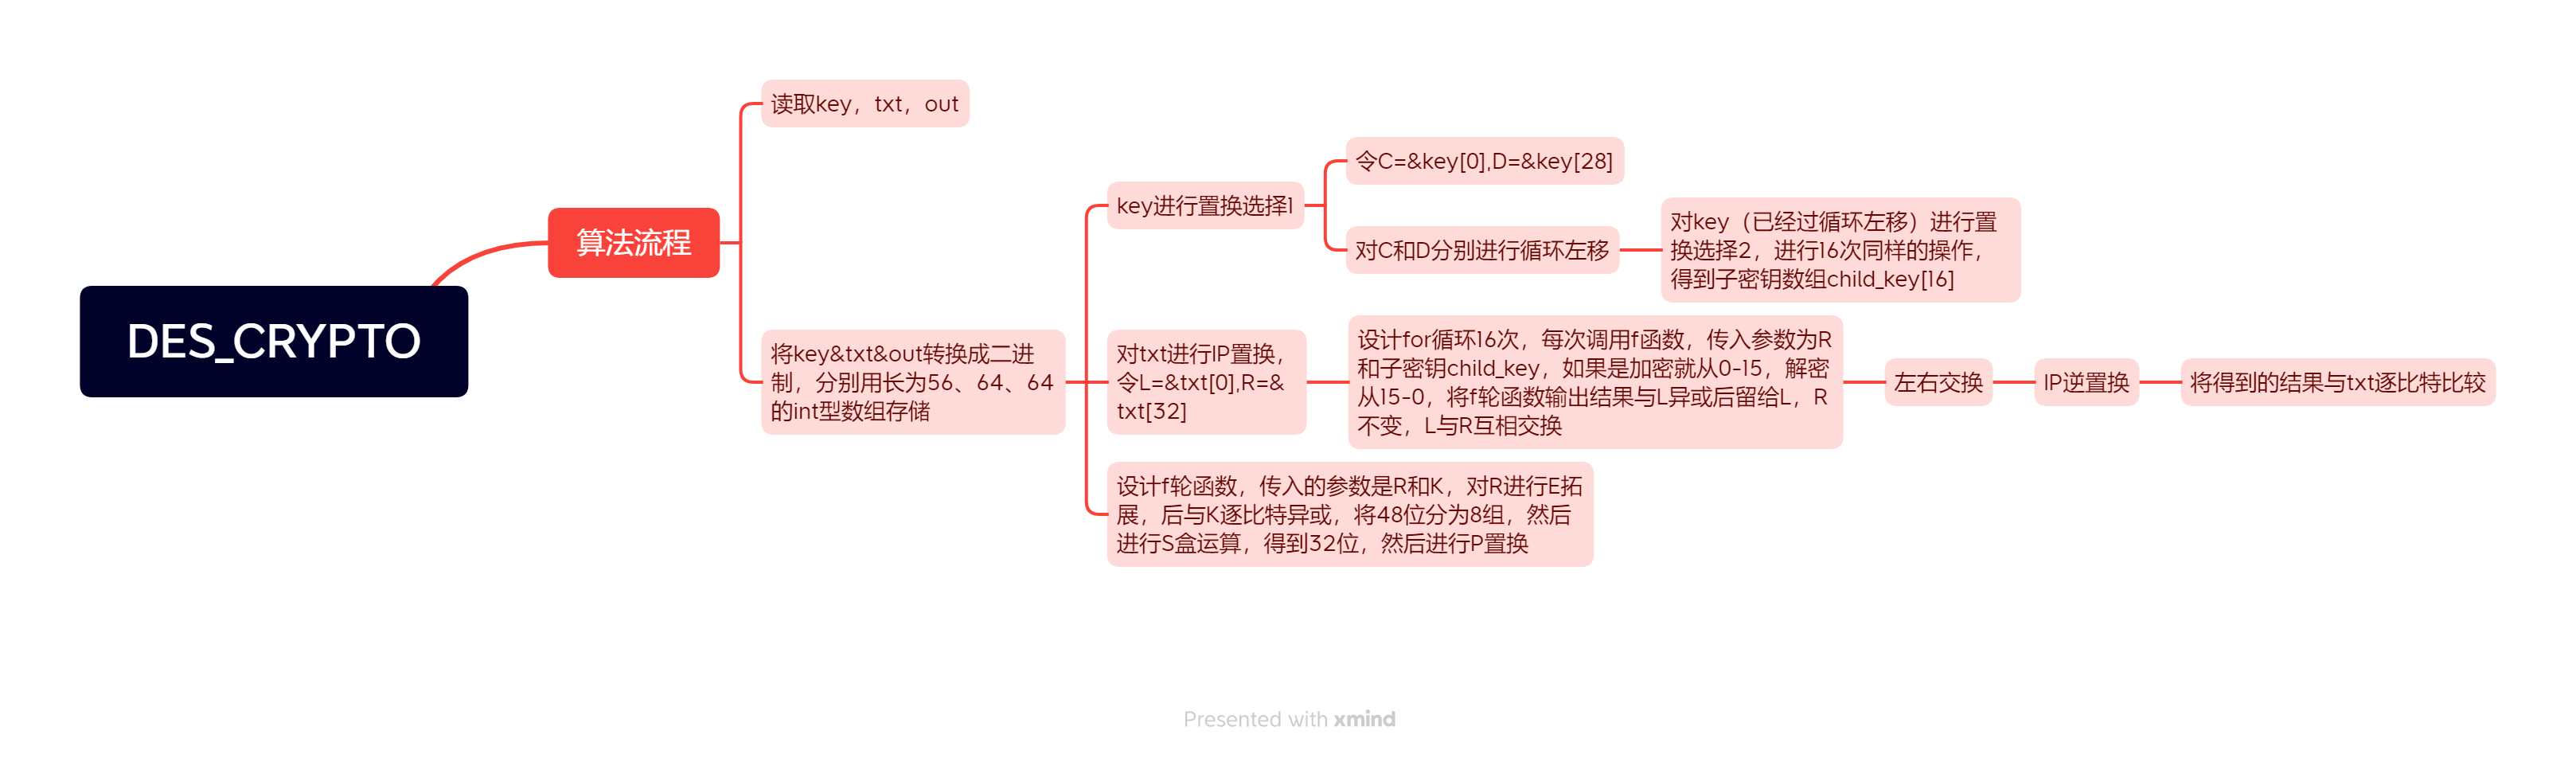
\includegraphics[height=6 CM,width=18cm]{figure/001}
	\caption{DES算法流程图}
	\label{fig:DES算法流程图}
\end{figure}
\begin{figure}[thbp!]
	\centering
	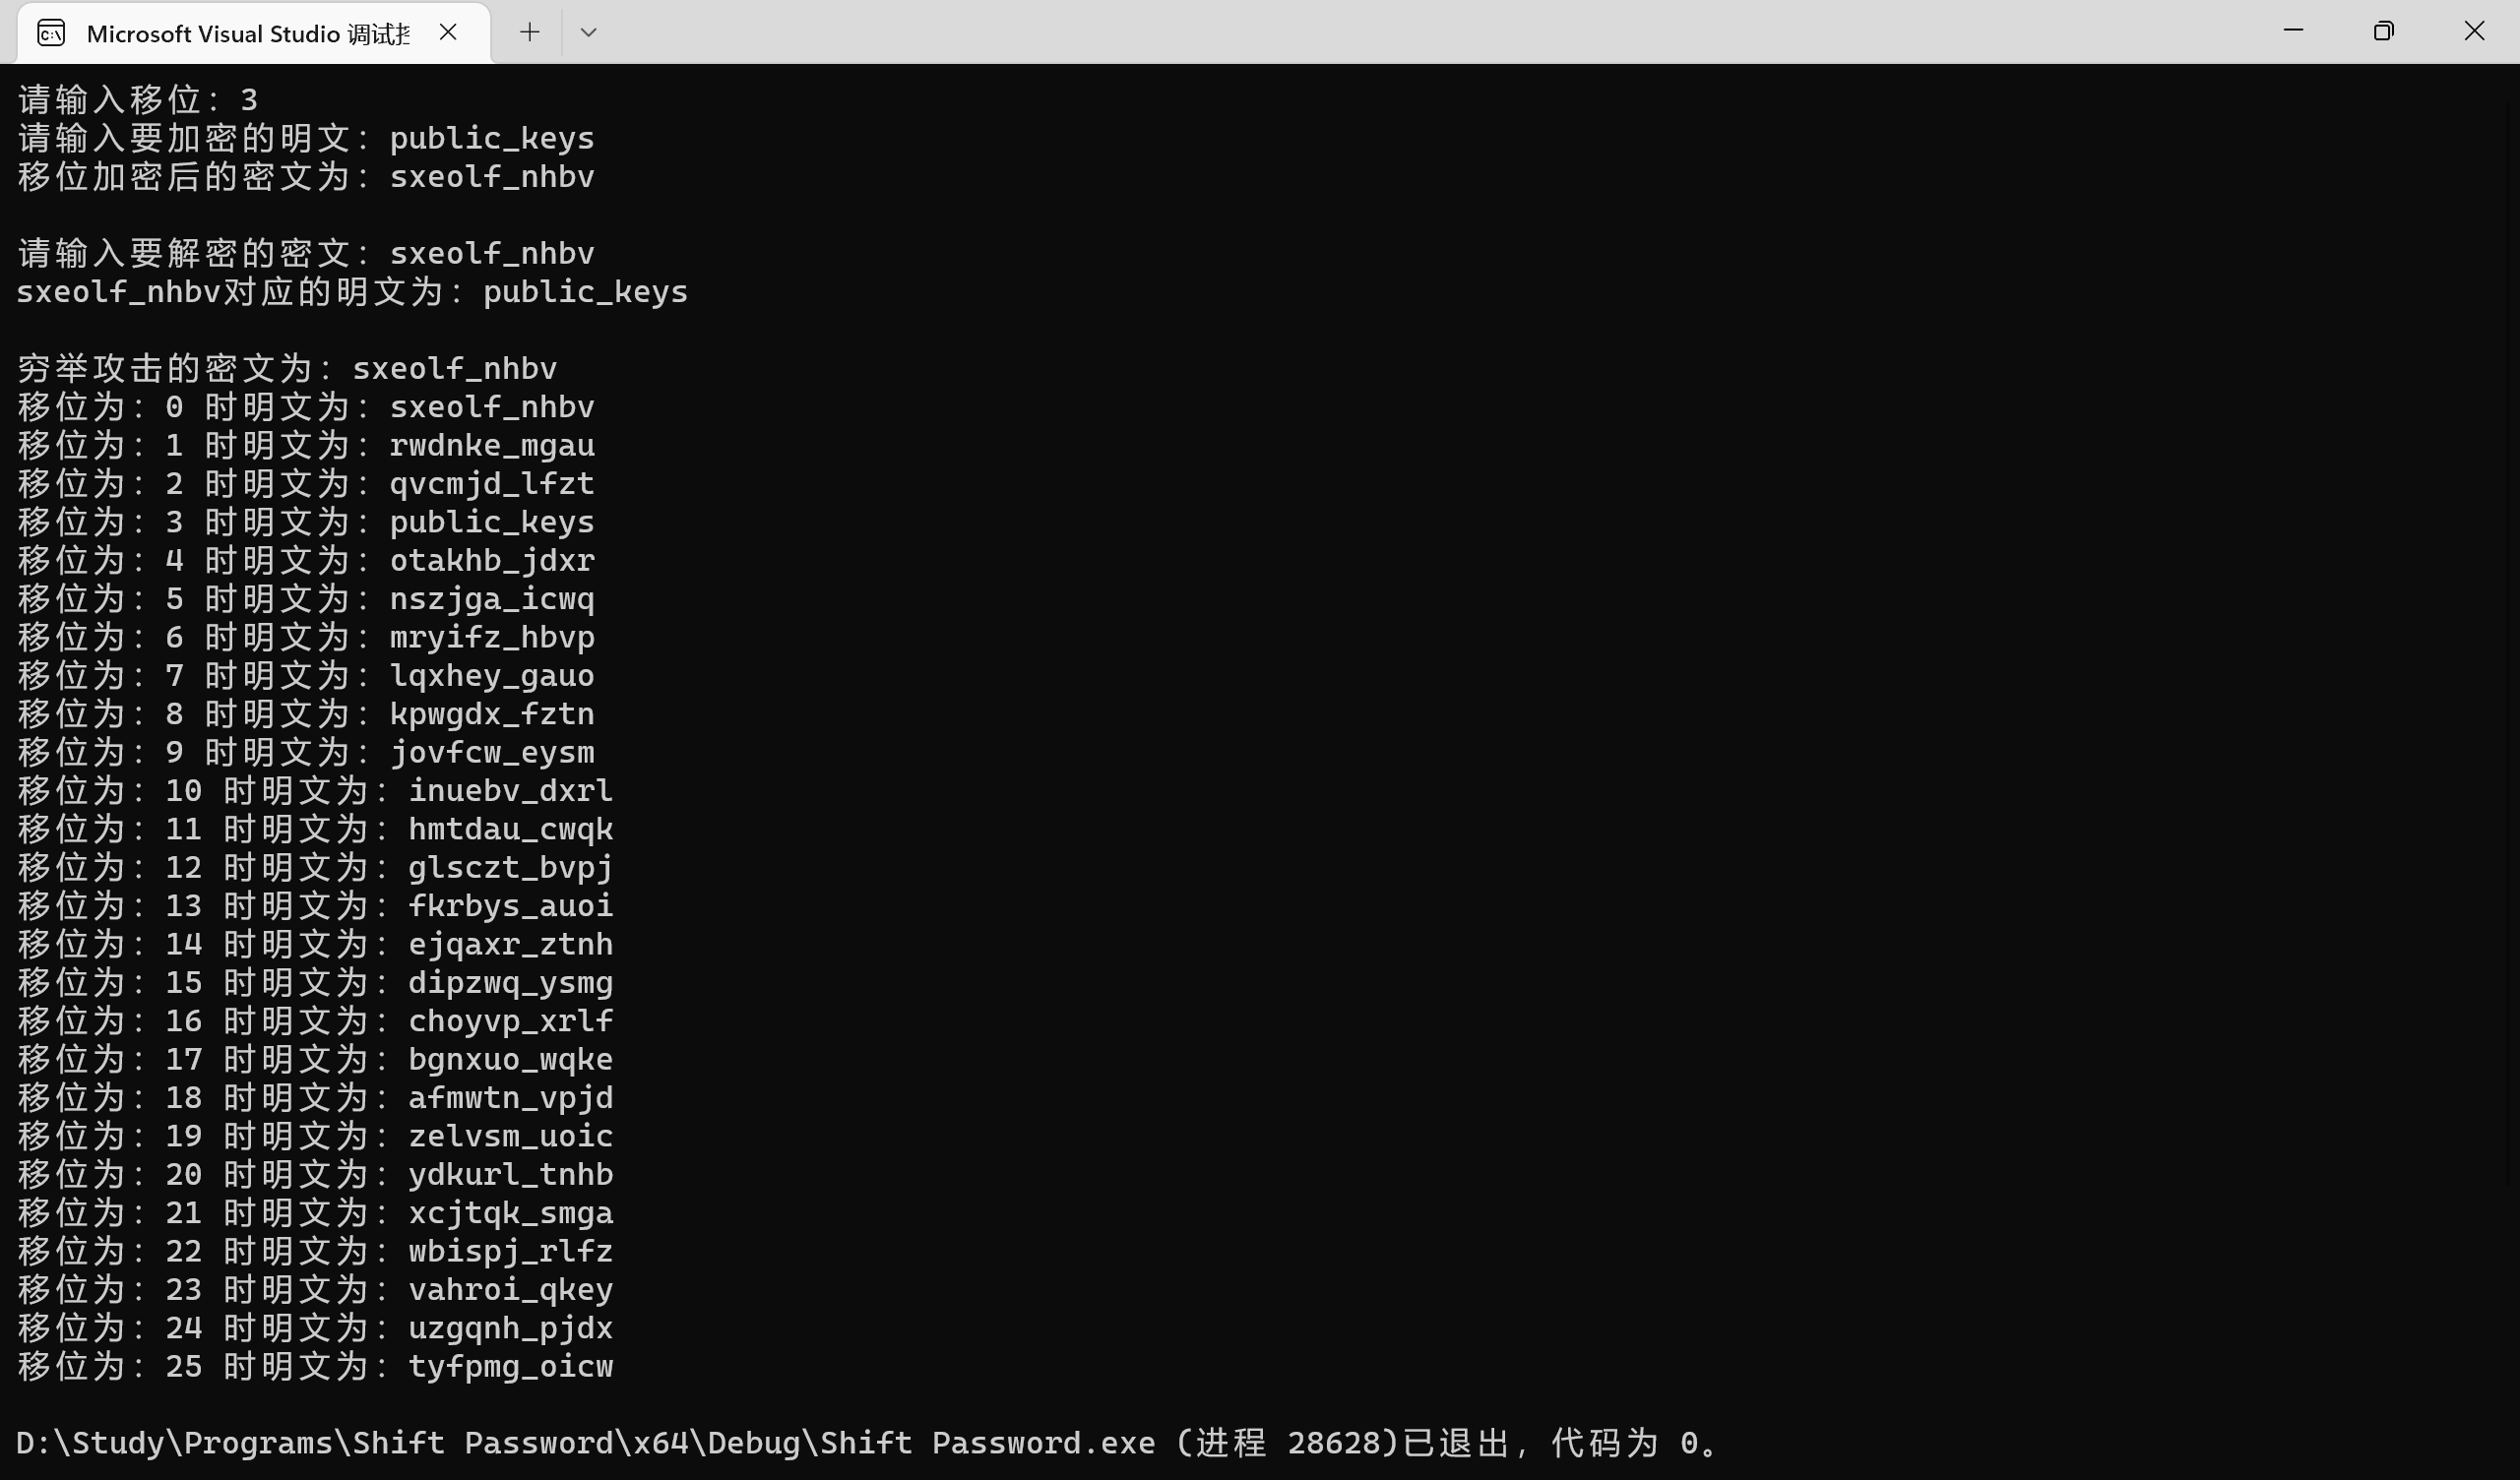
\includegraphics[height=10 CM]{figure/002}
	\caption{输出结果演示}
	\label{fig:输出结果演示}
\end{figure}

20组样例全部正确,改变key1位,8次得到的平均值是32,改变txt1位,8次计算得到的平均值是34\\

接下来概括性写一下中间生成结果(以第一组数据为例)\\
\begin{figure}[thbp!]
	\centering
	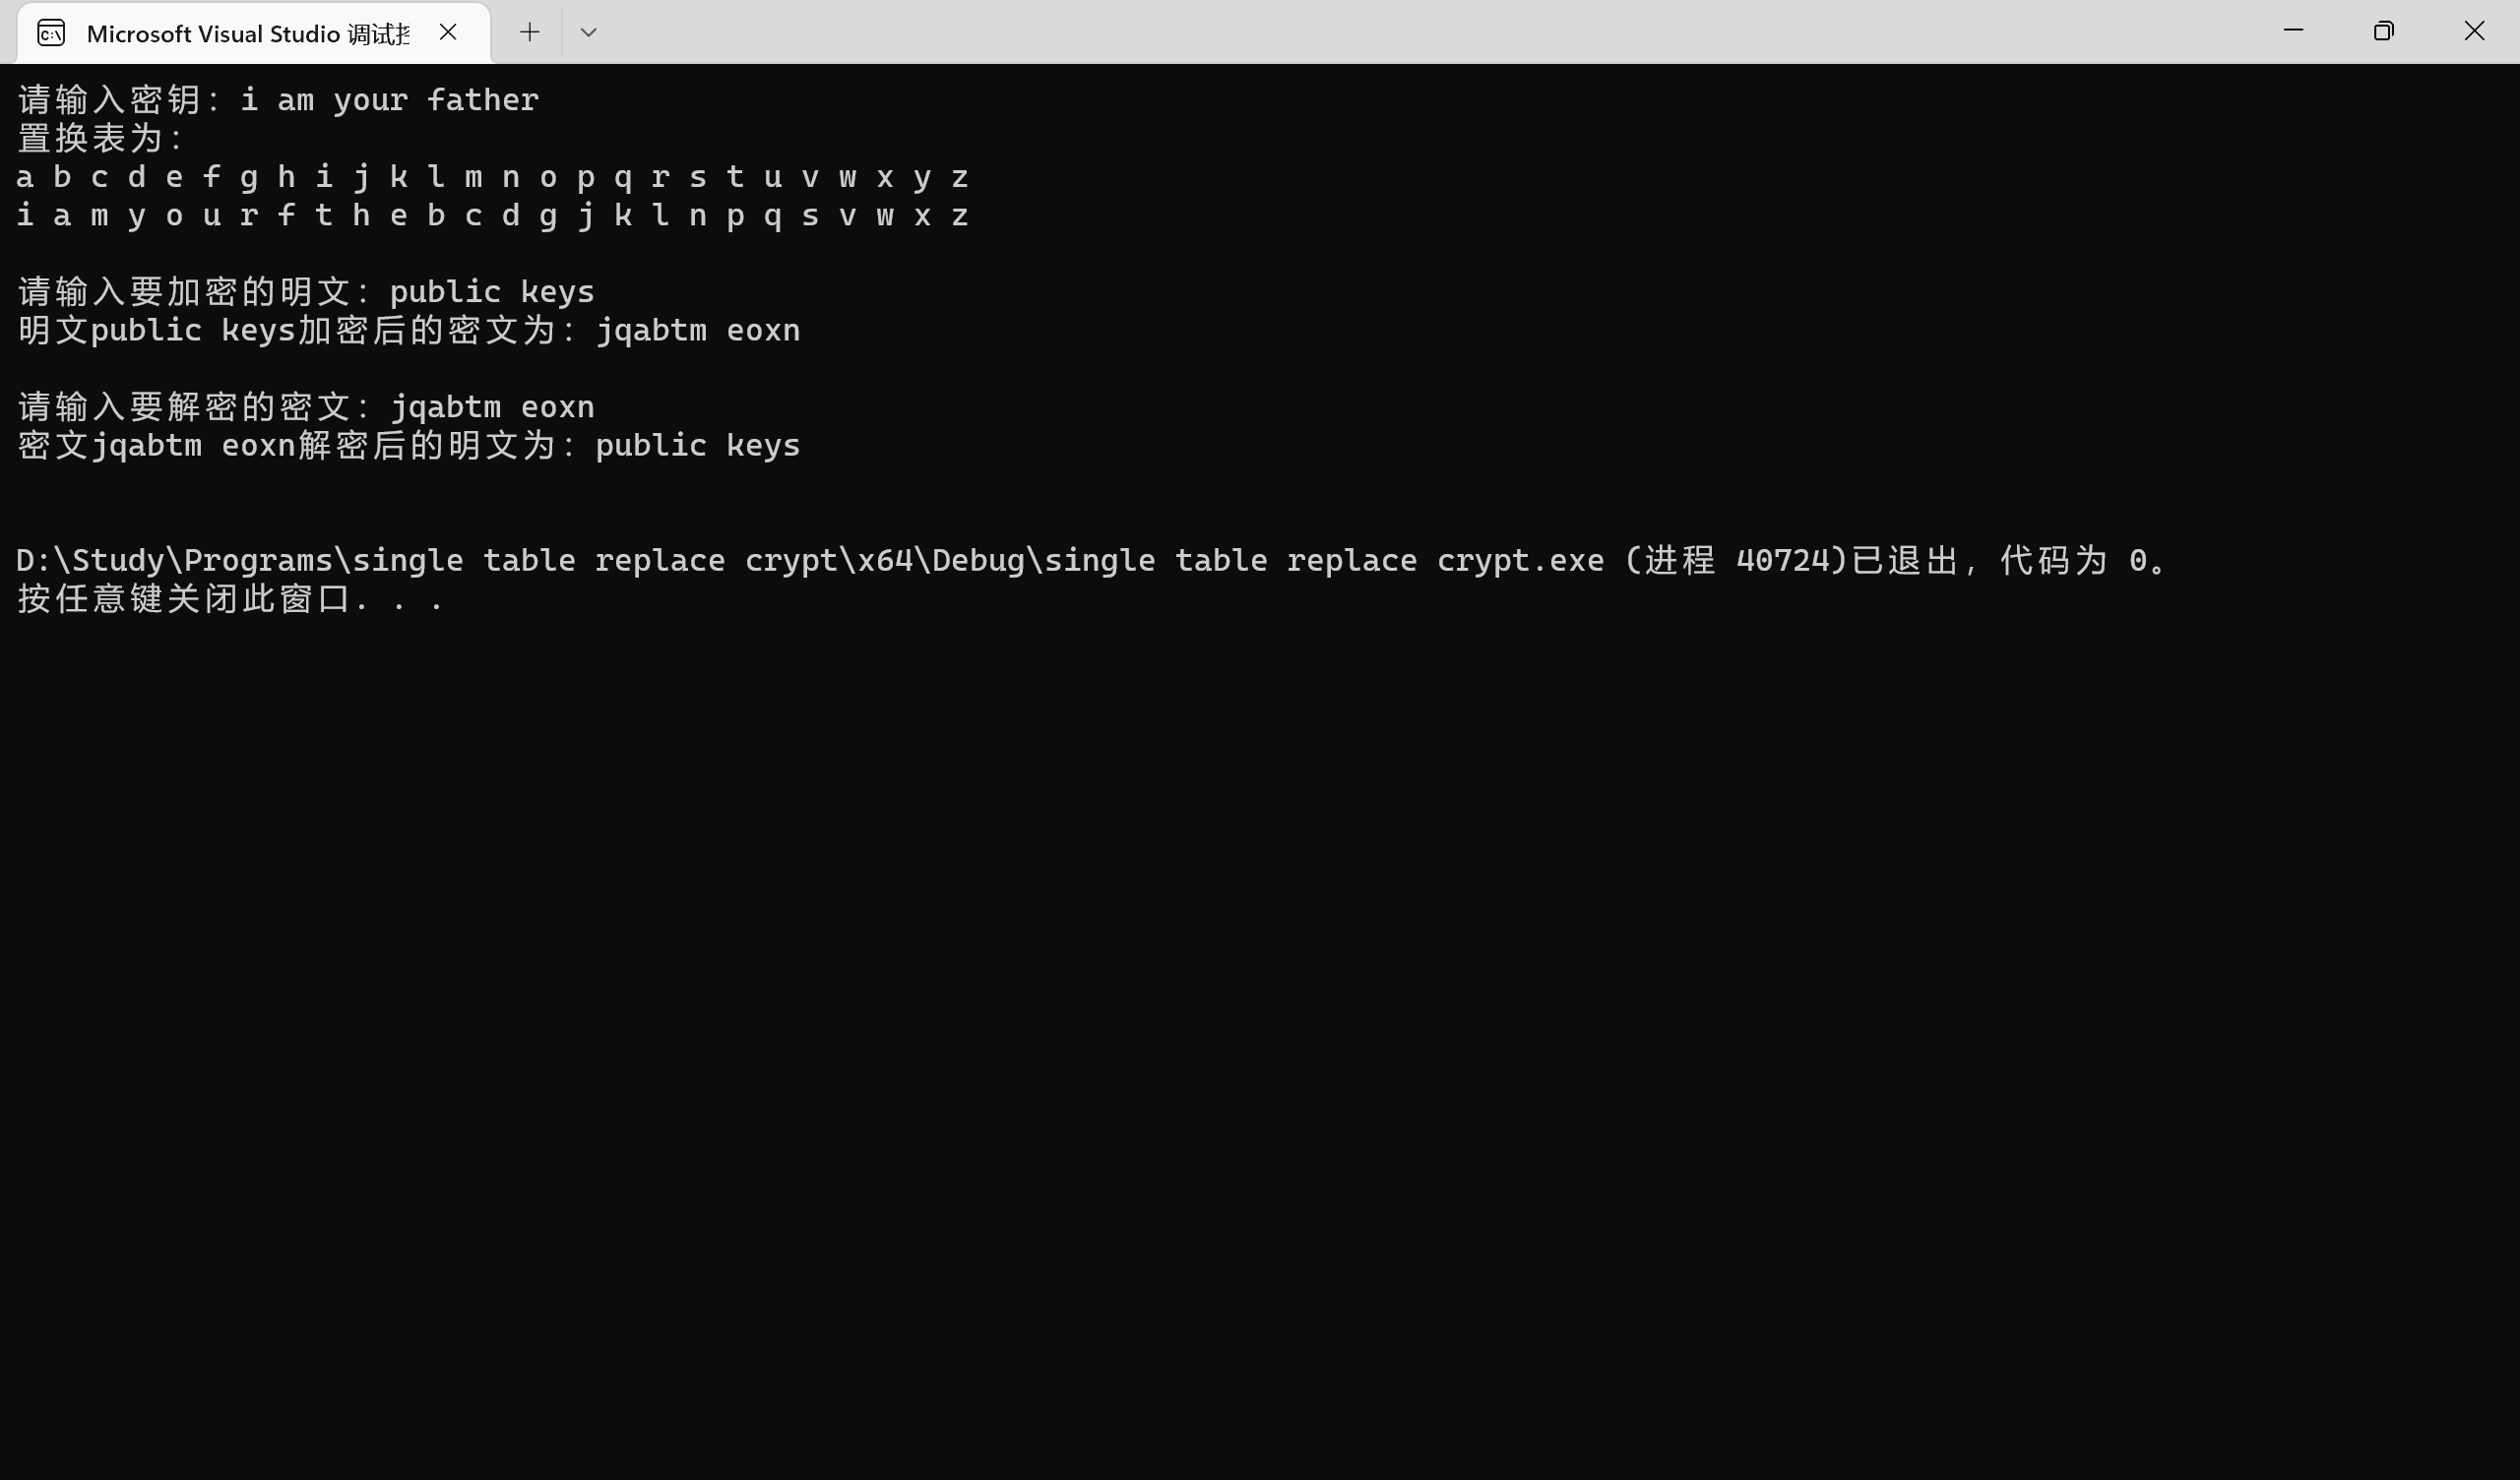
\includegraphics[height=10 CM]{figure/003}
	\caption{读入的第一组数据}
	\label{fig:读入的第一组数据}
\end{figure}
\begin{figure}[thbp!]
	\centering
	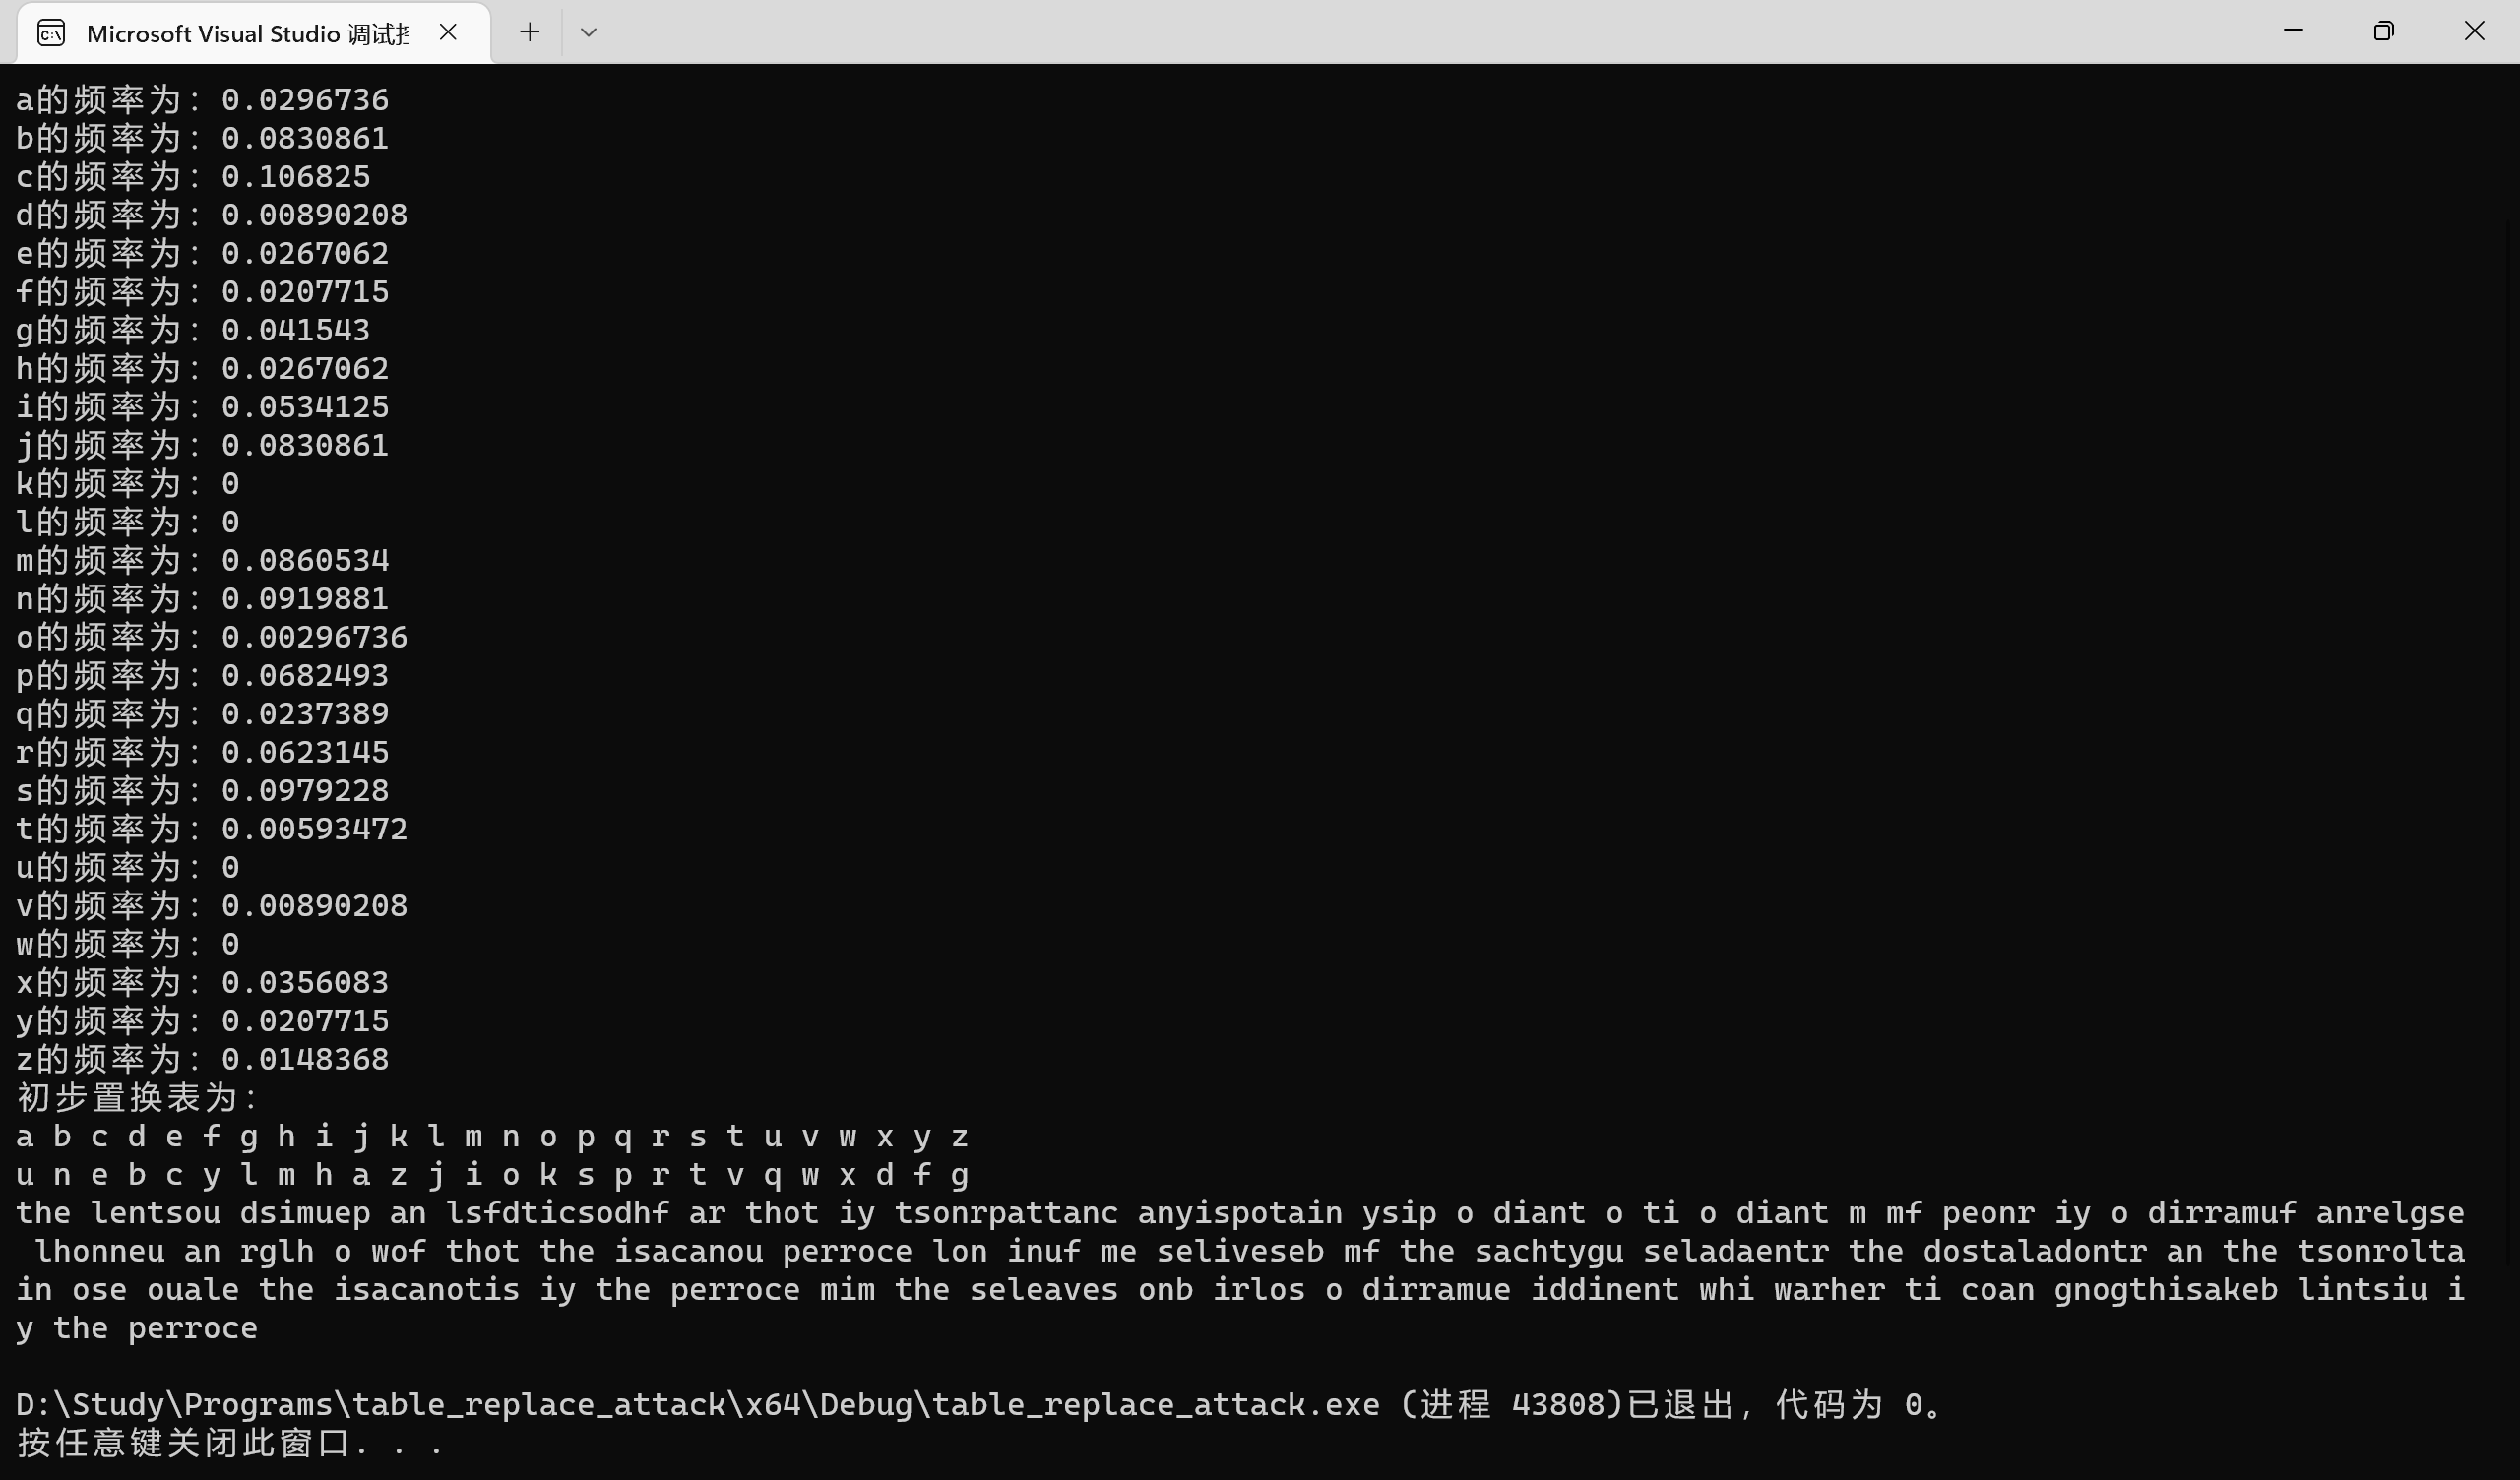
\includegraphics[height=10 CM]{figure/004}
	\caption{第一组计算结果与标准结果一致}
	\label{fig:第一组计算结果与标准结果一致}
\end{figure}
\begin{figure}[thbp!]
	\centering
	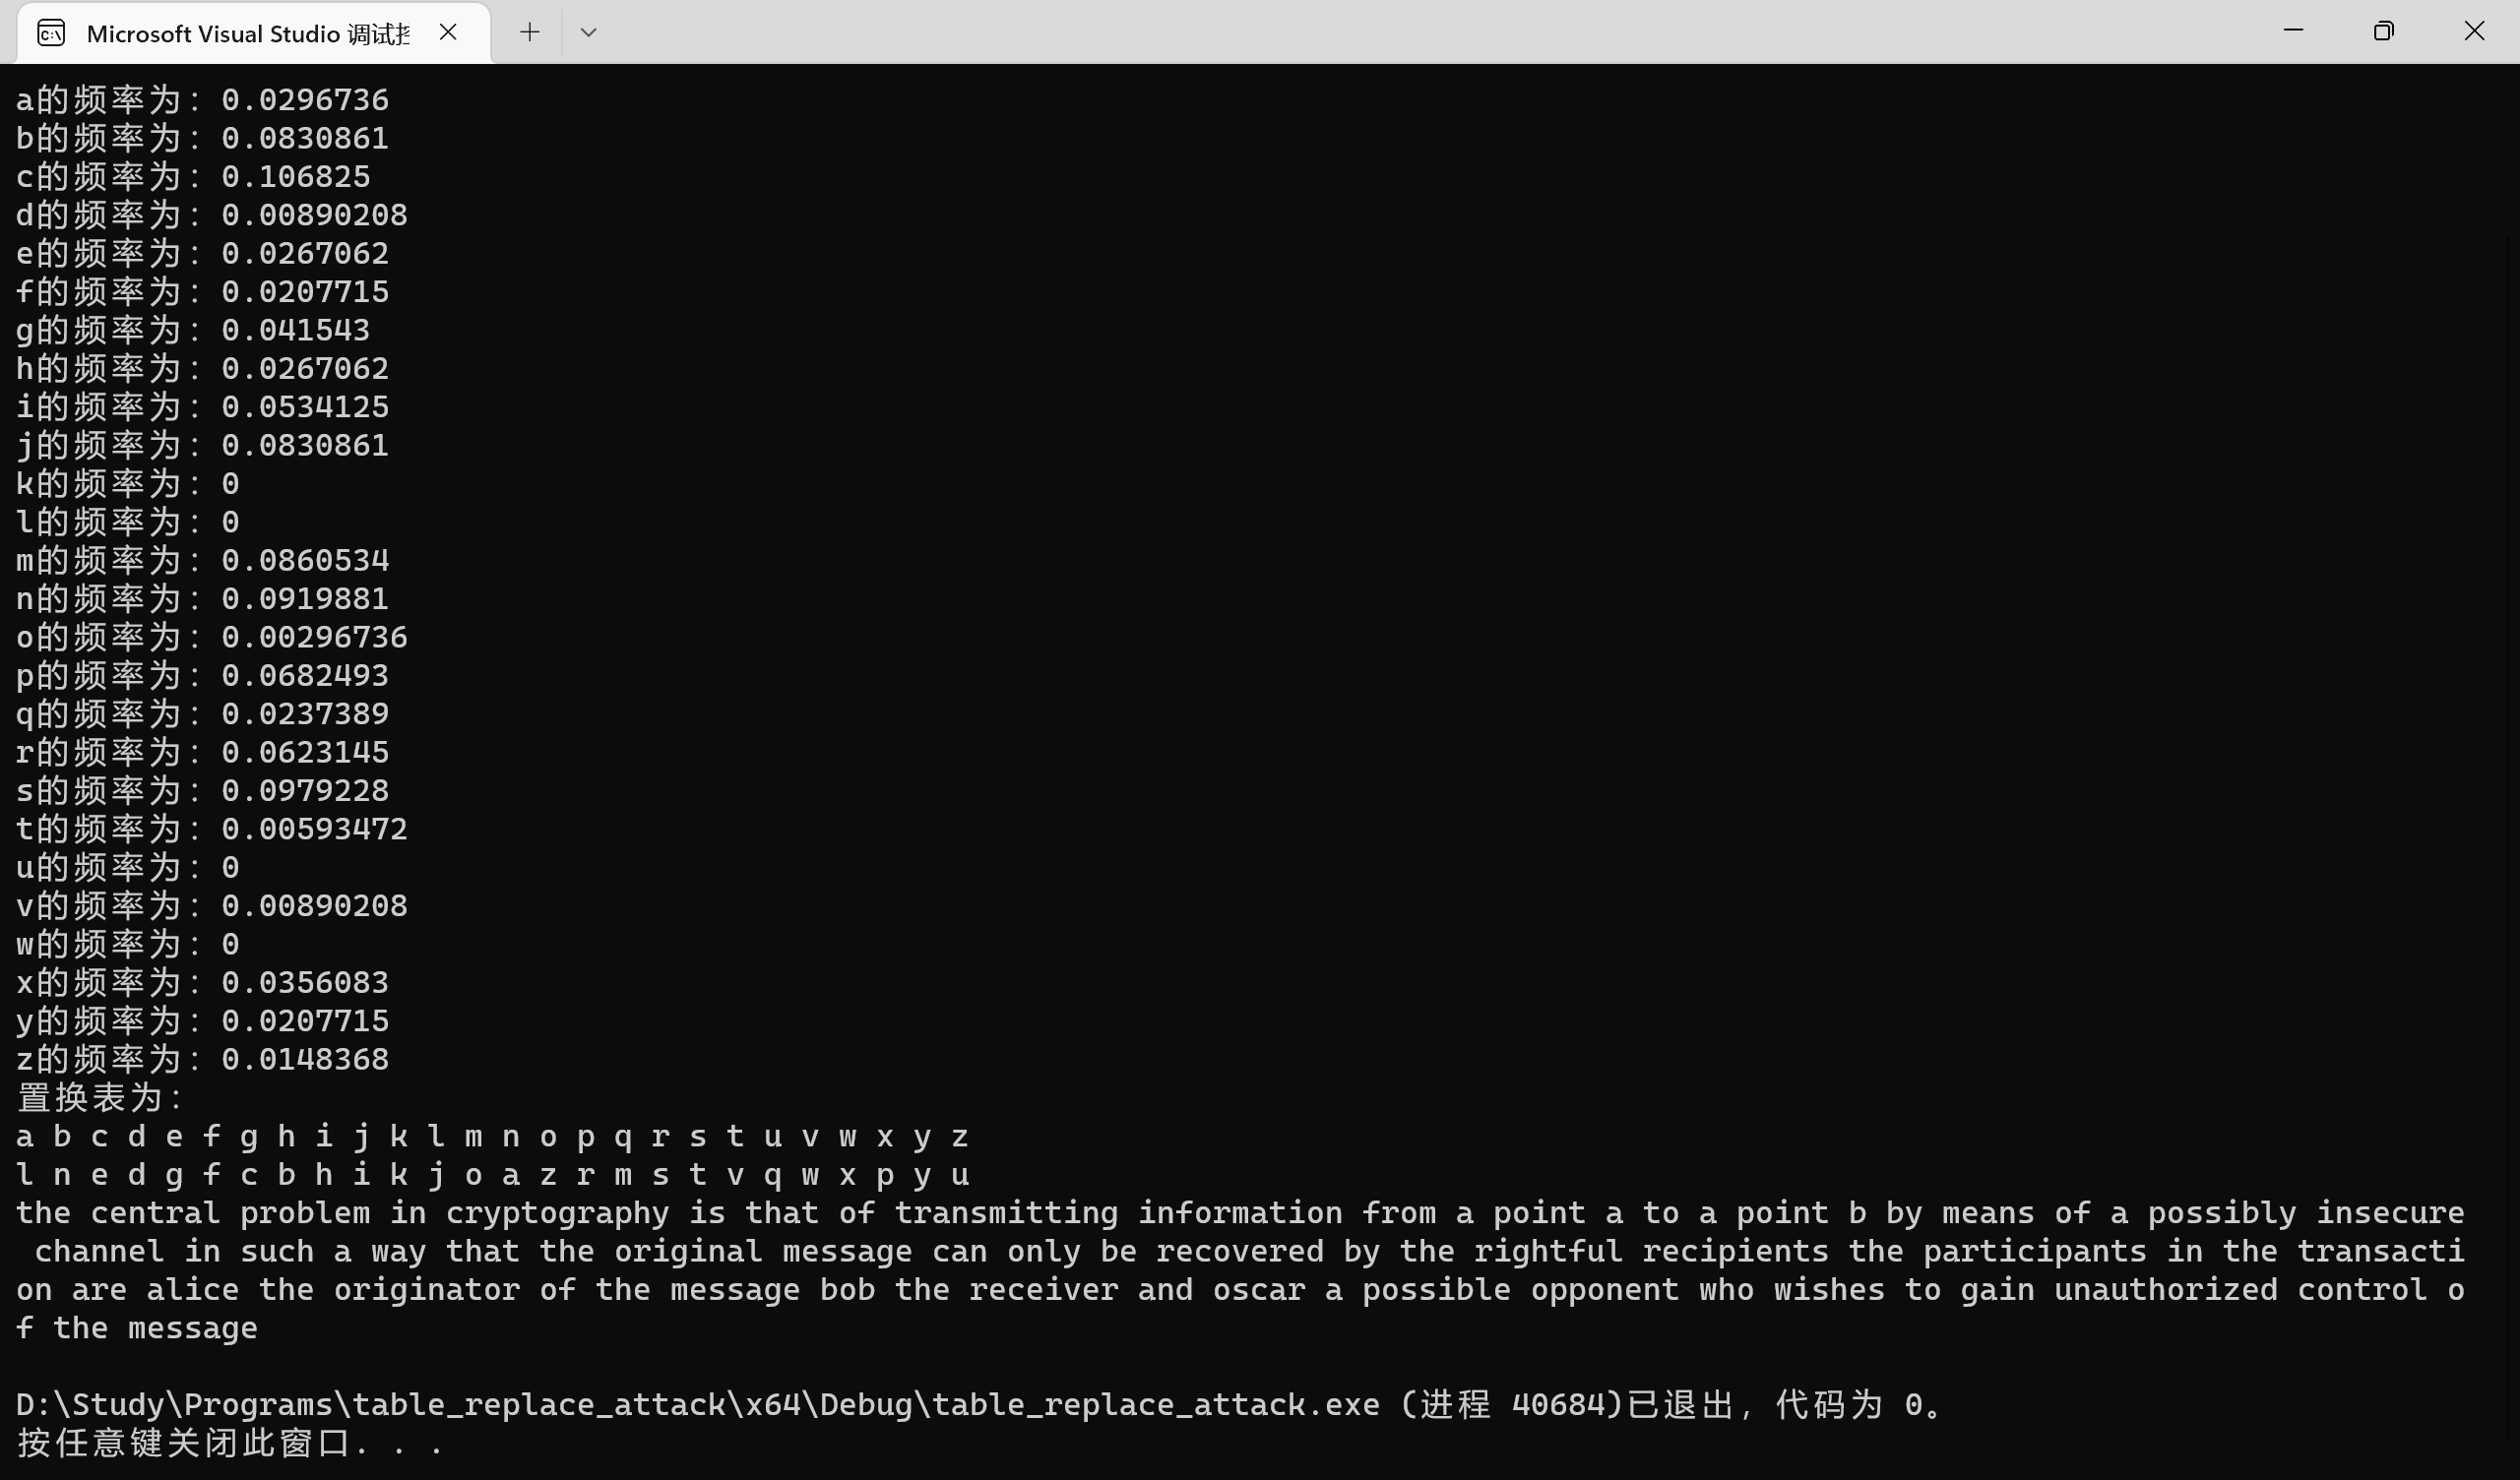
\includegraphics[height=10 CM]{figure/005}
	\caption{计算雪崩效应,改变key的一位,txt不变}
	\label{fig:计算雪崩效应,改变key的一位,txt不变}
\end{figure}
\begin{figure}[thbp!]
	\centering
	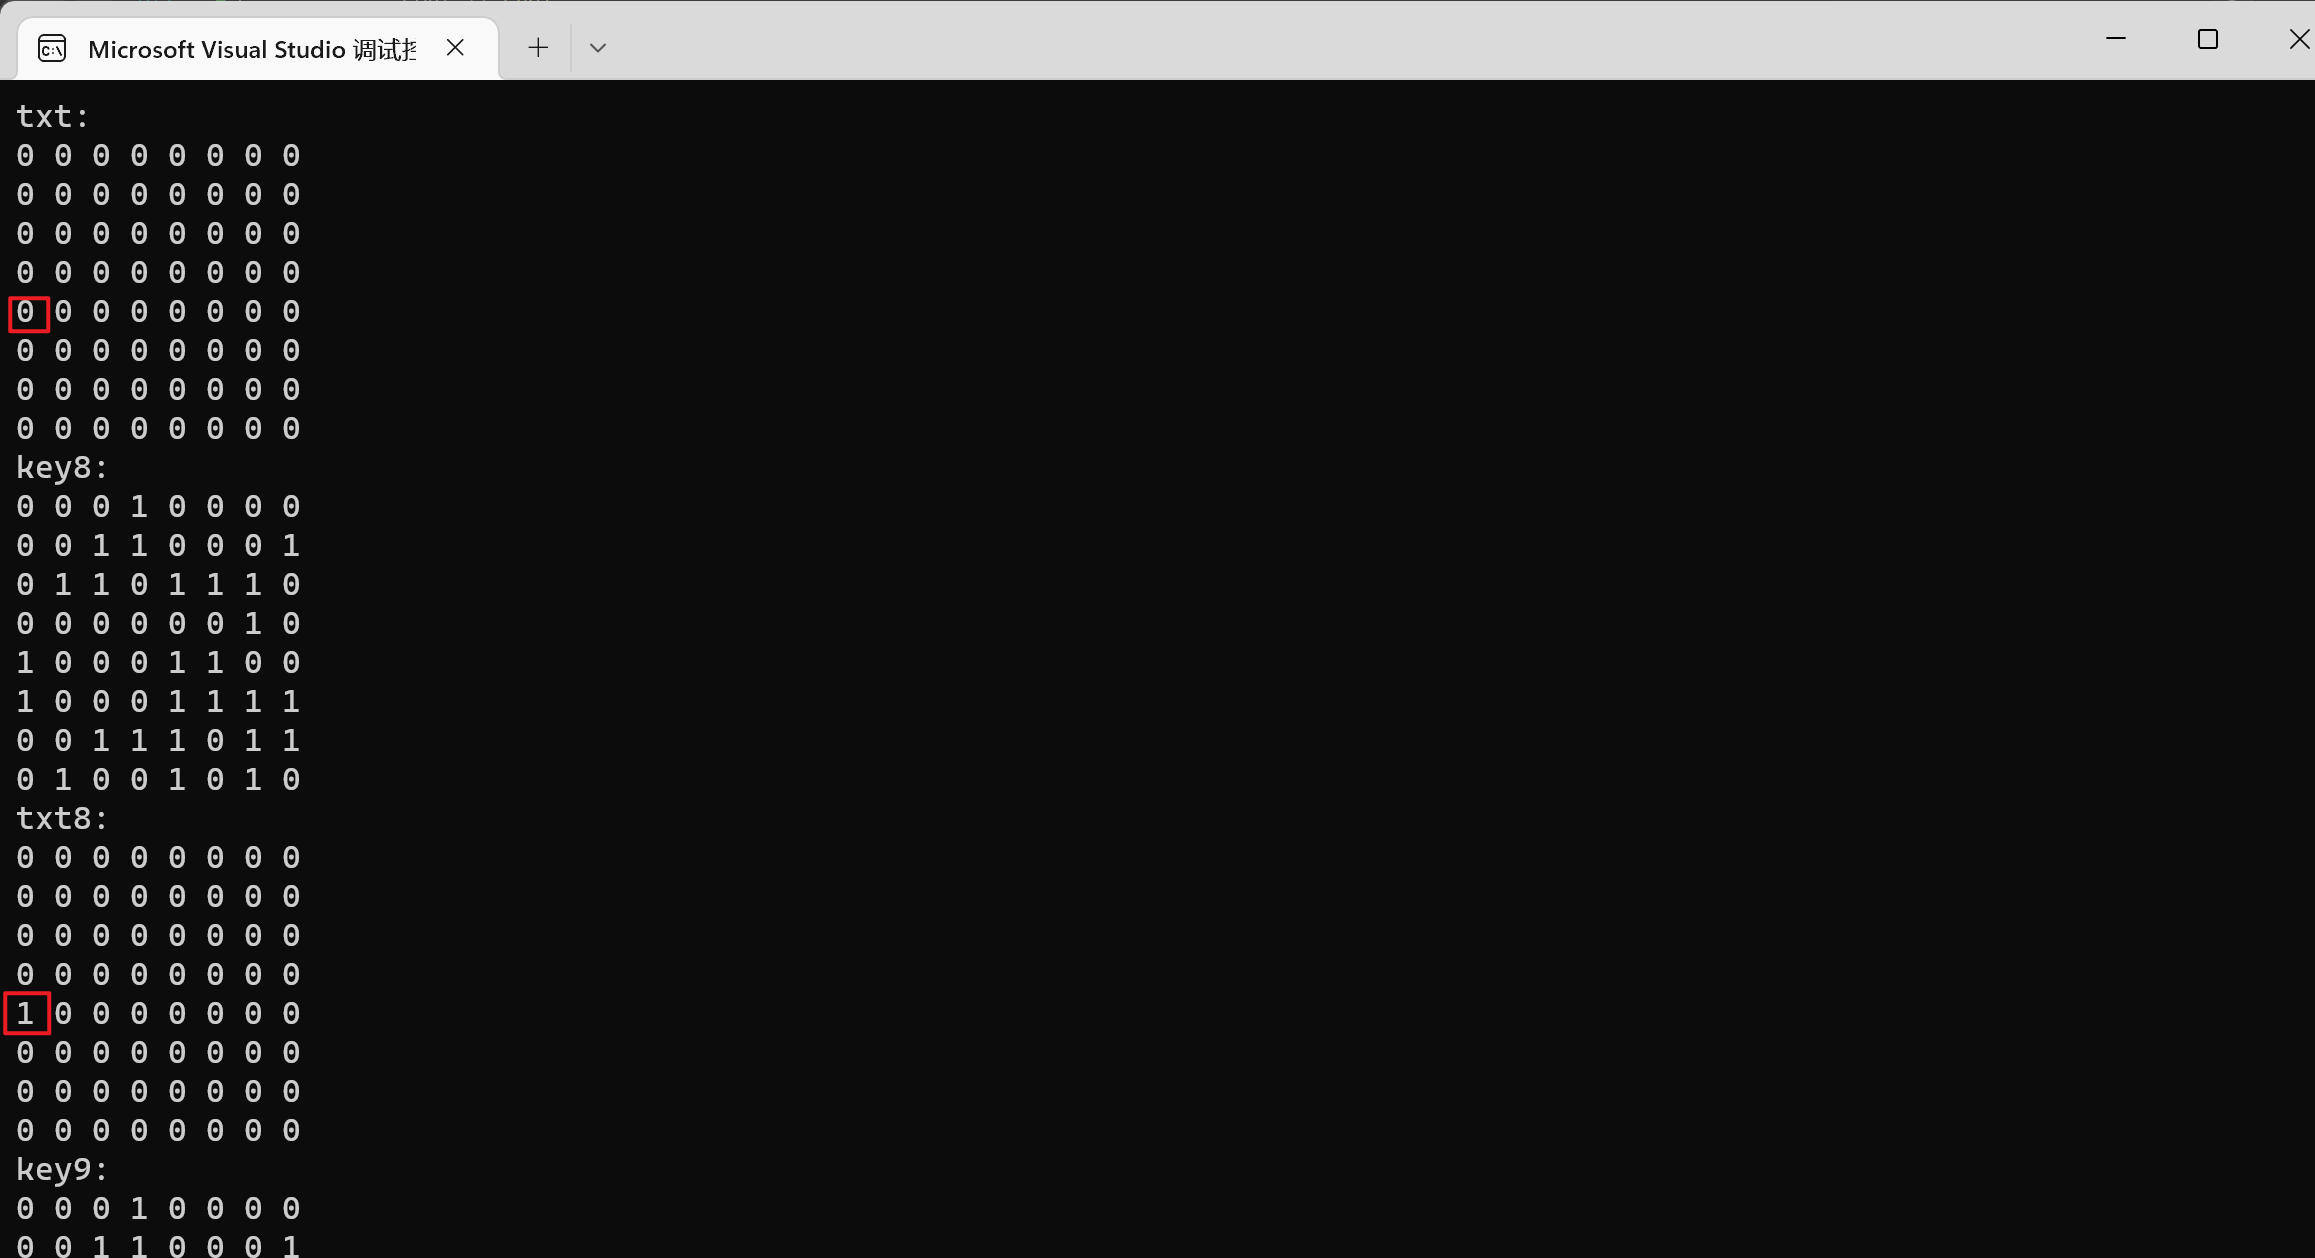
\includegraphics[height=10 CM]{figure/006}
	\caption{计算雪崩效应,改变txt的一位,key不变}
	\label{fig:计算雪崩效应,改变txt的一位,key不变}
\end{figure}
\begin{lstlisting}[language=c++]
// DES_CRYPTO.cpp : 
#include <iostream>
#include"des_test_data.h"
using namespace std;

int* child_key[16];//储存子密钥
//为了代码精简删掉表项,详情请见DES_CRYPTO.sln
const int IP_table[64] = {  };

const int IP_1_table[64] = { 
};
const int LS_table[16] = {
};
const int PC_1_table[56] = {};
const int PC_2_table[48] = { };
const int E_table[48] = { };
const int S_Box_table[32][16] = {  };
const int P_table[32] =
{
};

int* int2dec(int a)//a是int型,比如140
{
	int* b = new int[2];
	if (!a)
	b[0] = b[1] = 0;
	else
	{
		b[1] = a % 16;
		b[0] = a / 16;
	}
	return b;
}

void DEC2BIN(int a, int* b, int k)
{//将10进制数转换成2进制数,并用长度为4的int数组保存
	for (int i = 0; i < 8; i++)
	b[k + i] = 0;
	int* c = new int[2];
	c = int2dec(a);
	int temp;
	for (int i = 0; i < 2; i++)
	{
		if (!i)
		temp = k + 3;
		else
		temp = k + 7;
		while (c[i])
		{
			int j = c[i] % 2;
			c[i] /= 2;
			b[temp--] = j;
		}
	}
}

int* IP_replace(int* text)//IP置换
{
	int* temp = new int[64];
	for (int i = 0; i < 64; i++)
	{
		temp[i] = text[IP_table[i] - 1];
	}
	return temp;
}

int* IP_1_replace(int* text)//IP逆置换
{
	int* temp = new int[64];
	for (int i = 0; i < 64; i++)
	{
		temp[i] = text[IP_1_table[i] - 1];
	}
	return temp;
}

int* PC_1_replace(int* text)//压缩置换PC-1
{
	int k = 0;
	int* temp = new int[56];
	for (int i = 0; i < 56; i++)
	{
		temp[i] = text[PC_1_table[i] - 1];
	}
	return temp;
}

int* PC_2_replace(int* text)//压缩置换PC-2
{
	int* temp = new int[48];
	for (int i = 0; i < 48; i++)
	{
		temp[i] = text[PC_2_table[i] - 1];
	}
	return temp;
}

void LS(int* text,int K_num)
{//循环左移,K_num是第几个子密钥
	for (int j = 0; j < LS_table[K_num]; j++)
	{
		int* L = &text[0];
		int* R = &text[28];
		int temp1_1, temp1_2;
		temp1_1 = L[0], temp1_2 = R[0];
		for (int i = 0; i < 27; i++)
		{
			L[i] = L[i + 1];
			R[i] = R[i + 1];
		}
		L[27] = temp1_1;
		R[27] = temp1_2;
	}
}

int* f(int* R, int* K)
{
	int* temp = new int[48];
	for (int i = 0; i < 48; i++)
	{
		temp[i] = R[E_table[i] - 1];//E拓展
		if (temp[i] == K[i])//E拓展后与子密钥异或
		temp[i] = 0;
		else
		temp[i] = 1;
	}
	int* tmp = new int[32];
	for (int i = 0; i < 32; i++)
	tmp[i] = 0;
	for (int s = 0; s < 8; s++)//s代表盒号
	{
		int k = s * 6;
		//i,j用来定位在盒里的坐标s[i][j]
		int i= temp[k] * 2 + temp[k + 5];
		int j = temp[k + 1] * 8 + temp[k + 2] * 4
		 + temp[k + 3] * 2 + temp[k + 4];
		int num = S_Box_table[s * 4 + i][j];
		int N = s * 4 + 3;
		while (num)
		{
			int i = num % 2;
			num /= 2;
			tmp[N--] = i;
		}
	}
	int* tmpp = new int[32];
	for (int i = 0; i < 32; i++)
	{
		tmpp[i] = tmp[P_table[i] - 1];
	}
	return tmpp;
}

int main()
{
	//保存第0组数据,用于后续雪崩检验
	int key0[64], txt0[64], out0[64];
	cout << "num" << "\tmode" << endl;
	//20组数据,前10组为加密,后10组为解密
	for (int i = 0; i < 20; i++)
	{
		int k = 0;
		int* key = new int[64];//储存密钥
		int* txt = new int[64];//储存txt
		int* output = new int[64];//DES计算的结果
		int* out = new int[64];//正确的结果
		
		
//将key,txt,out转换成2进制,共64位,存储在长位64的int型数组里面
		for (int j = 0; j < 8; j++)
		{
			DEC2BIN((int)cases[i].key[j], key, k);
			DEC2BIN((int)cases[i].txt[j], txt, k);
			DEC2BIN((int)cases[i].out[j], out, k);
			k += 8;
		}
		//保存第0组的数据,用于后续雪崩效应的计算
		if (i == 0)
		{
			for (int i = 0; i < 64; i++)
			{
				key0[i] = key[i];
				txt0[i] = txt[i];
			}
		}
		int* temp = PC_1_replace(key);//压缩置换1
		for (int i = 0; i < 16; i++)
		{
			//循环左移
			LS(temp, i);
			//压缩置换2
			child_key[i] = PC_2_replace(temp);
		}
		txt = IP_replace(txt);//IP置换
		int* L = &txt[0];
		int* R = &txt[32];
		int j;//j用来区分加密和解密使用的子密钥不同
		if (cases[i].mode)
		{
			j = 0;
		}
		else
			j = 15;
		for (int k = 0; k < 16; k++)//16轮
		{
			int* tmpp;
			if (cases[i].mode)
			{//加密,子密钥正序使用0-15
				tmpp = f(R, child_key[j++]);
			}
			else//解密,子密钥逆序使用15-0
				tmpp = f(R, child_key[j--]);
			for (int i = 0; i < 32; i++)
			{//Ri=Li-1+f(Ri-1,Ki)
				if (tmpp[i] == L[i])
					L[i] = 0;
				else
					L[i] = 1;
			}
			int* temp = L;
			L = R;
			R = temp;
		}
		for (int i = 0; i < 32; i++)//左右交换
		{
			swap(L[i], R[i]);
		}
		output = IP_1_replace(txt);//IP逆置换
		if (i == 0)
		{
			for (int i = 0; i < 64; i++)
			{
				out0[i] = output[i];
			}
		}
	//用来判断计算得到的output与标准答案out是否一致
		bool t = true;
		for (int k = 0; k < 64; k++)
		{
			if (out[k] != output[k])
			{
				t = false;//不一致
				break;
			}
		}
		if (t)
			cout << cases[i].num << " \t" <<
			 cases[i].mode << "  \t成功" << endl;
		else
			cout << cases[i].num << " \t" << 
			cases[i].mode << "  \t失败" << endl;
	}
	
	//测试雪崩效应,选取第一组数据
	int num = 0;
//计算16次,前8次计算改变1bit密钥,不改变明文
//后8次计算改变1bit明文,不改变密钥
	for (int i = 0; i < 16; i++)
	{
		if (i % 8 == 0)
		num = 0;
		int* testkey = new int[64];
		int* testtxt = new int[64];
		int* testout = new int[64];
		if (i < 8)
		{
			for (int j = 0; j < 64; j++)
			{
				if (j == i * 8)
				{
					testkey[j] = (key0[j] + 1) % 2;
				}
				else
				{
					testkey[j] = key0[j];
				}
				testtxt[j] = txt0[j];
			}
		}
		else
		{
			for (int j = 0; j < 64; j++)
			{
				if (j == i * 4)
				{
					testtxt[j] = (txt0[j] + 1) % 2;
				}
				else
				{
					testtxt[j] = txt0[j];
				}
				testkey[j] = key0[j];
			}
		}
		int* temp = PC_1_replace(testkey);
		for (int i = 0; i < 16; i++)
		{
			LS(temp, i);
			child_key[i] = PC_2_replace(temp);
		}
		testtxt = IP_replace(testtxt);
		int* L = &testtxt[0];
		int* R = &testtxt[32];
		for (int k = 0; k < 16; k++)
		{
			int* tmpp;
			tmpp = f(R, child_key[k++]);
			for (int i = 0; i < 32; i++)
			{
				if (tmpp[i] == L[i])//Ri=Li-1+f(Ri-1,Ki)
				L[i] = 0;
				else
				L[i] = 1;
			}
			int* temp = L;
			L = R;
			R = temp;
		}
		for (int i = 0; i < 32; i++)//左右交换
		{
			swap(L[i], R[i]);
		}
		testout = IP_1_replace(testtxt);
		for (int i = 0; i < 64; i++)
		{
			if (out0[i] != testout[i])
			num++;
		}
		if (i == 7)
			cout << "The average of out changed 
			for changed 1bit of key is " <<
			 float(num / 8) << endl;
		if (i == 15)
			cout << "The average of out changed 
			for changed 1bit of txt is " <<
			 float(num / 8) << endl;
	}
}

\end{lstlisting}
%\begin{enumerate}
%	\item \textbf {预处理器:}处理源代码中以\#开始的预编译指令,例如展开所有宏定义、插入\#include指向的文件等,以获得经过预处理的源程序。
%	
%	\item \textbf {编译器:}将预处理器处理过的源程序文件翻译成为标准的汇编语言以供计算机阅读。
%	
%	\item \textbf {汇编器:}将汇编语言指令翻译成机器语言指令,并将汇编语言程序打包成可重定位目标程序。
%	
%	\item \textbf {链接器:}将可重定位的机器代码和相应的一些目标文件以及库文件连接在一起,形成真正能在机器上运行的目标机器代码。
%\end{enumerate}

%\begin{figure}[thbp!]
%	\centering
%	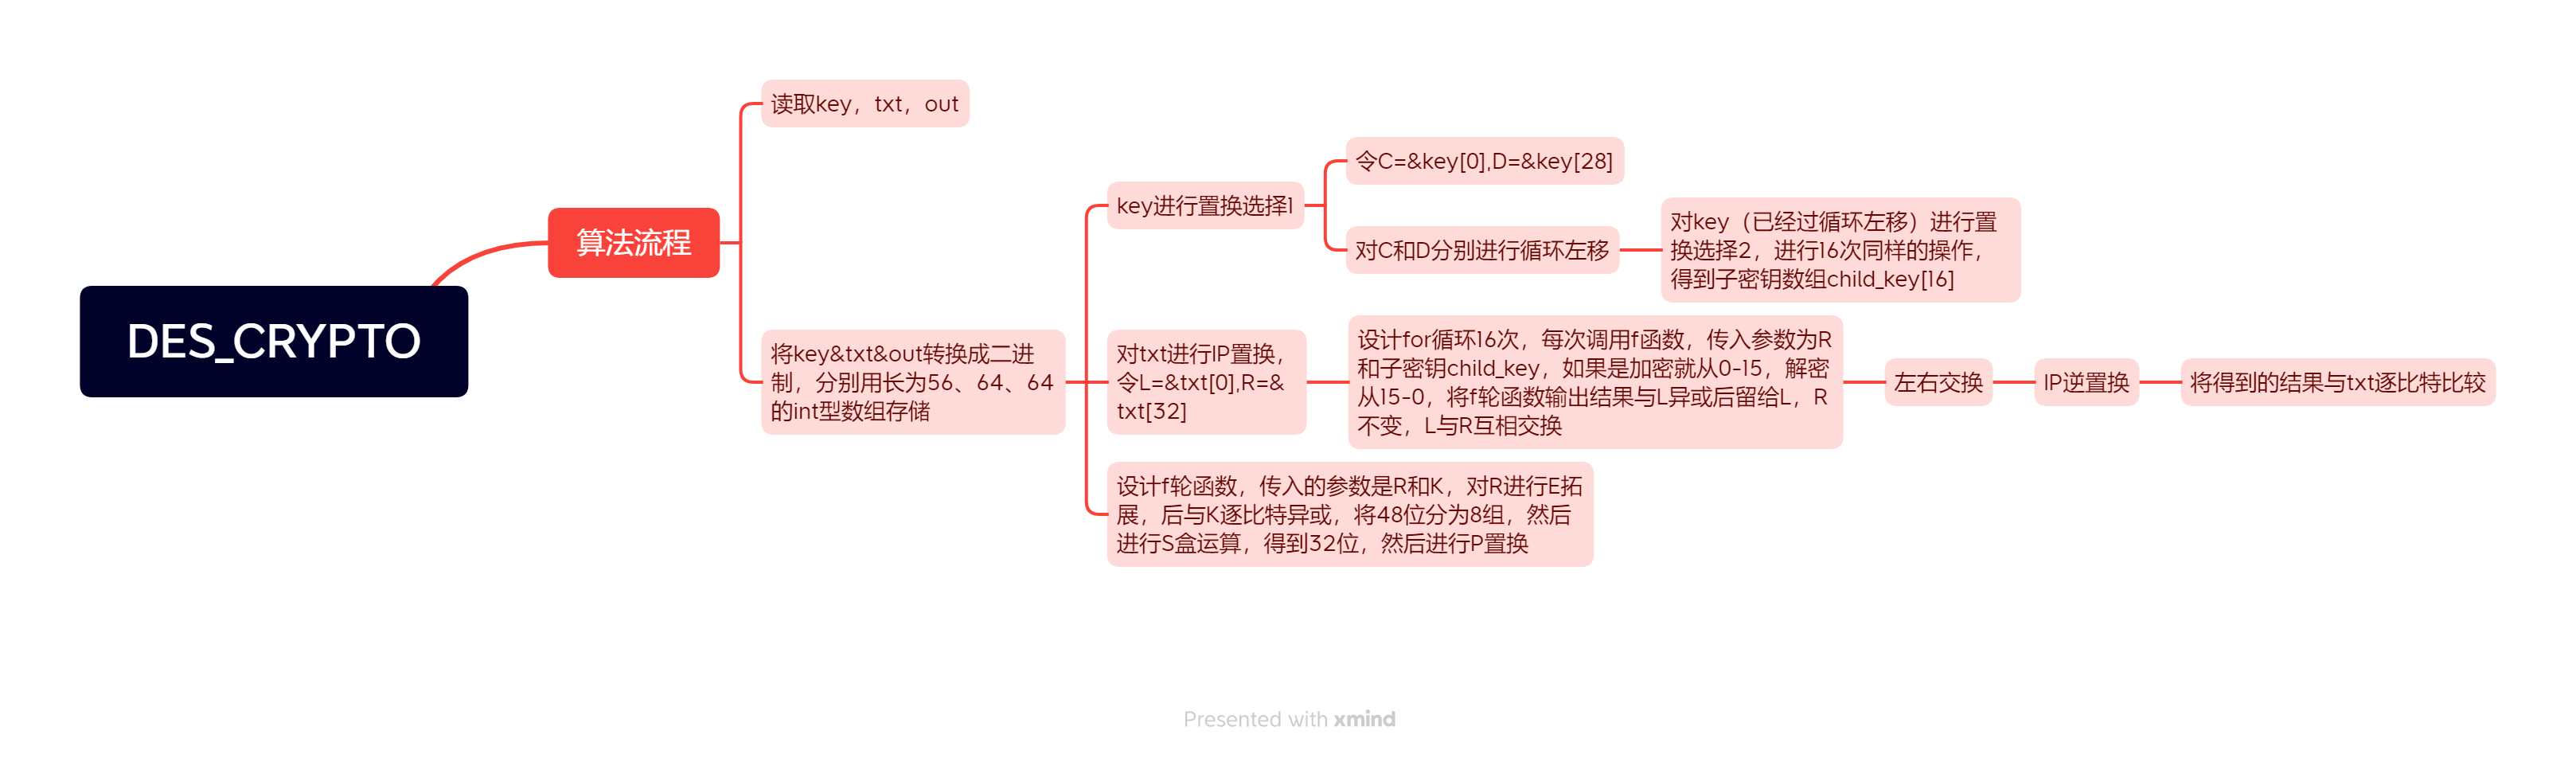
\includegraphics[height=6.8 CM]{figure/001}
%	\caption{语言处理过程图示}
%	\label{fig:语言处理过程图示}
%\end{figure}

























      %
	\pagenumbering{arabic}
\section{单表置换密码的加解密}

\subsection{单表置换密码的加解密流程}
\begin{figure}[thbp!]
	\centering
	
\includegraphics[width=16cm]{figure/figure2.png}
	\caption{单表置换密码的加解密流程}
	\label{fig:单表置换密码的加解密流程}
\end{figure}

\subsection{单表置换密码程序代码}
\begin{lstlisting}[language=c++]
#include <iostream>
#include<string.h>
using namespace std;

//处理输入的密钥
int* build_table(char* inputtext)
{
	int len = strlen(inputtext);
	//输入的密钥长度大于26,则只取前26个
	if (len > 26)
	{
		inputtext[26] = '\0';
		len = 26;
	}
	int* temp = new int[26];
	int j = 0;
	temp[j] = -1;
	for (int i = 0; i < len; i++)
	{
		if (inputtext[i] >= 'A' && inputtext[i] <= 'Z')
		{
			inputtext[i] = inputtext[i] - 'A' + 'a';
		}
		if (inputtext[i] >= 'a' && inputtext[i] <= 'z')
		{
			bool t = true;
			int n = inputtext[i] - 'a';
			for (int k = 0; k <= j; k++)
			{
				if (temp[k] == n)
				{
					t = false;
					break;
				}
			}
			if (t)
			{
				temp[j] = n;
				j++;
			}
		}
	}
	for (int i = 0; i < 26; i++)
	{
		bool t = true;
		for (int k = 0; k < j; k++)
		{
			if (temp[k] == i)
			{
				t = false;
				break;
			}
		}
		if (!t)
			continue;
		else
		{
			temp[j] = i;
			j++;
		}
	}
	//for (int i = 0; i < 26; i++)
	//{
	//    cout << temp[i] << " ";
	//}
	return temp;
}

//解密时使用
int retnum(int* replacetable, int num)
{
	for (int i = 0; i < 26; i++)
	{
		if (replacetable[i] == num)
		{
			return i;
		}
	}
}

class table_replace_crypt
{
private:
	int* replacetable = new int[26];//置换表
public:
	table_replace_crypt()
	{
		for (int i = 0; i < 26; i++)
		{
			replacetable[i] = i;
		}
	}
	table_replace_crypt(char* input)
	{
		replacetable = build_table(input);
	}
	int* getreplacetable()
	{
		return replacetable;
	}
	char* table_replace_encrypt(char*plaintext)//加密
	{
		int len = strlen(plaintext);
		char* ciphertext = new char[len];
		for (int i = 0; i < len; i++)
		{
			if (plaintext[i] >= 'a' && plaintext[i] <= 'z')
			{
				int n = plaintext[i] - 'a';
				ciphertext[i] = plaintext[i] + replacetable[n] - n;
			}
			else if (plaintext[i] >= 'A' && plaintext[i] <= 'Z')
			{
				int n = plaintext[i] - 'A';
				ciphertext[i] = plaintext[i] + replacetable[n] - n;
			}
			else
			ciphertext[i] = plaintext[i];
		}
		ciphertext[len] = '\0';
		return ciphertext;
	}
	char* table_replace_decrypt(char* ciphertext)//解密
	{
		int len = strlen(ciphertext);
		char* plaintext = new char[len];
		for (int i = 0; i < len; i++)
		{
			if (ciphertext[i] >= 'a' && ciphertext[i] <= 'z')
			{
				int n = retnum(replacetable, ciphertext[i] - 'a');
				plaintext[i] = 'a' + n;
			}
			else if (ciphertext[i] >= 'A' && ciphertext[i] <= 'Z')
			{
				int n = retnum(replacetable, ciphertext[i] - 'A');
				plaintext[i] = 'A' + n;
			}
			else
			plaintext[i] = ciphertext[i];
		}
		plaintext[len] = '\0';
		return plaintext;
	}
};
int main()
{
	
	cout << "请输入密钥:";
	char* input = new char[24];
	cin.getline(input, 20);
	
	table_replace_crypt pro = table_replace_crypt(input);
	cout << "置换表为:" << endl;
	for (int i = 0; i < 26; i++)
	{
		cout << char('a' + i) << " ";
	}
	cout << endl;
	int* temp = pro.getreplacetable();
	for (int i = 0; i < 26; i++)
	{
		cout << char('a' + temp[i]) << " ";
	}
	cout << endl << endl;
	
	cout << "请输入要加密的明文:";
	char* plaintext = new char[24];
	char* temp1;
	cin.getline(plaintext, 20);
	temp1 = pro.table_replace_encrypt(plaintext);
	cout << "明文" << plaintext << "加密后的密文为:" << temp1 << endl << endl;
	
	cout << "请输入要解密的密文:";
	char* ciphertext = new char[24];
	char* temp2;
	cin.getline(ciphertext, 20);
	temp2 = pro.table_replace_decrypt(ciphertext);
	cout << "密文" << ciphertext << "解密后的明文为:" << temp2 << endl << endl;
	return 0;
}
\end{lstlisting}


\subsection{程序运行结果}
\begin{figure}[thbp!]
	\centering
	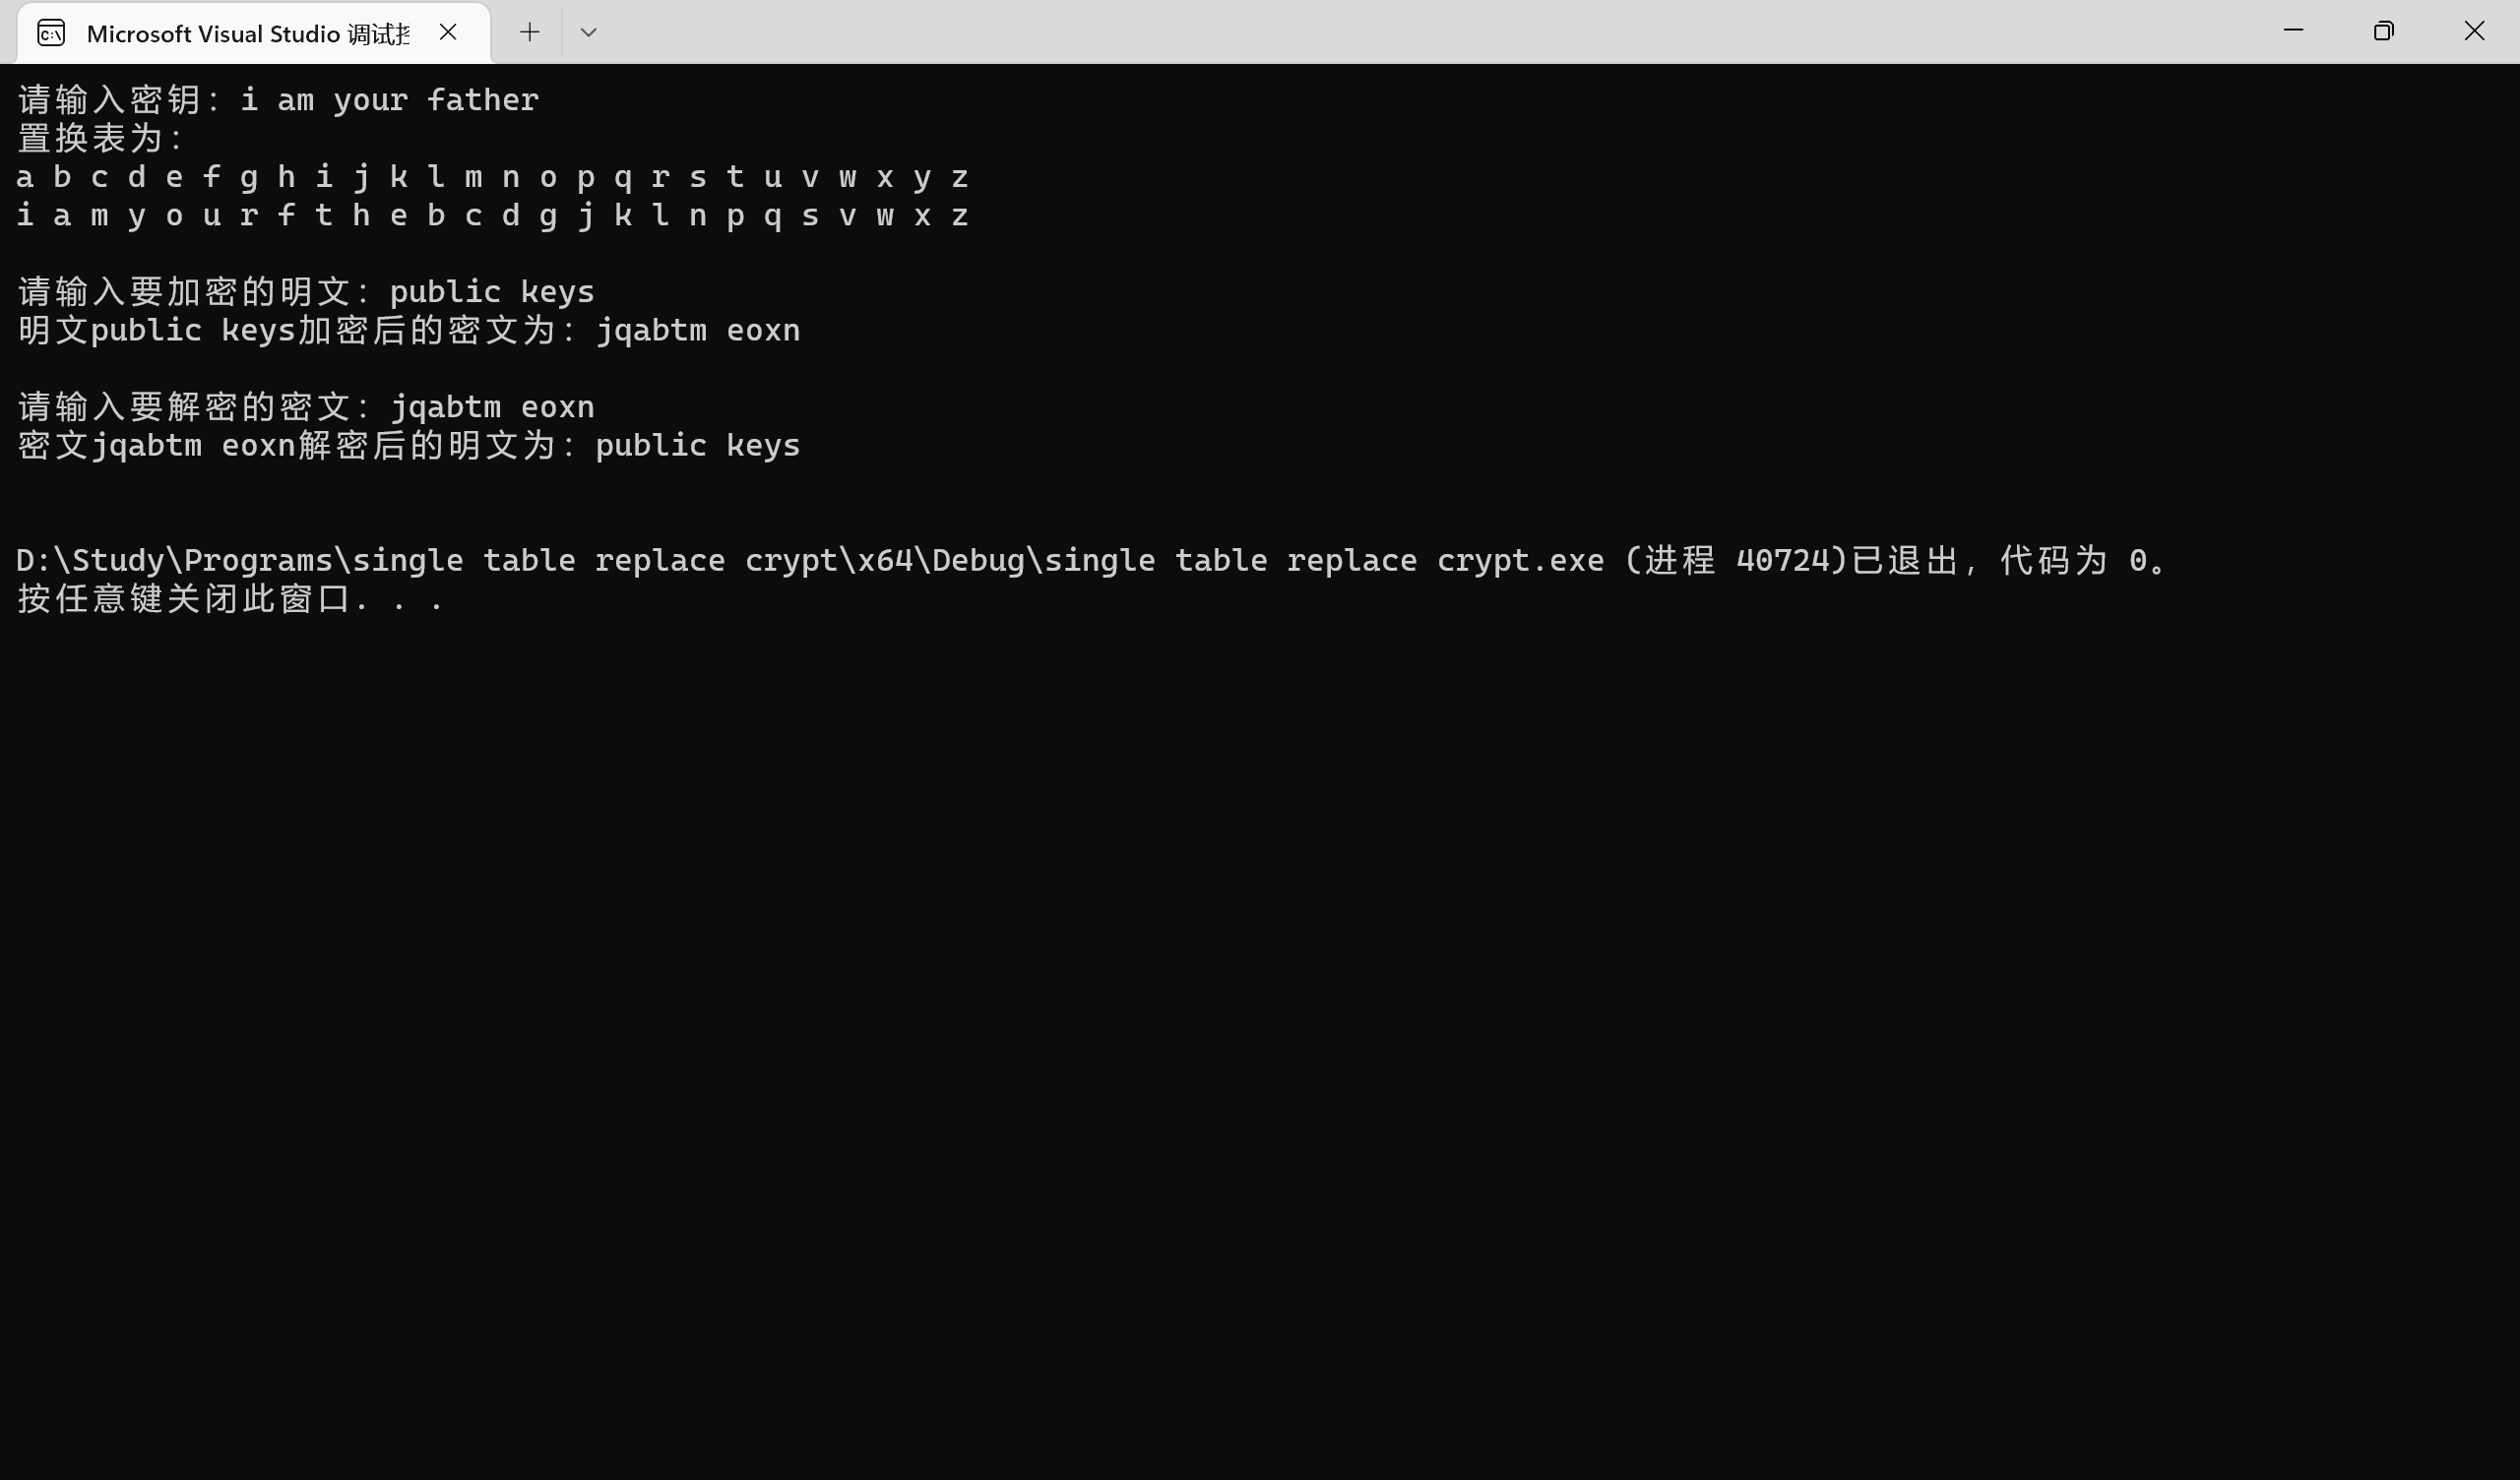
\includegraphics[width=16cm]{figure/003.png}
	\caption{单表置换密码加解密程序运行结果}
	\label{fig:单表置换密码加解密程序运行结果}
\end{figure}

%\begin{enumerate}
%	\item \textbf {预处理器:}处理源代码中以\#开始的预编译指令,例如展开所有宏定义、插入\#include指向的文件等,以获得经过预处理的源程序。
%	
%	\item \textbf {编译器:}将预处理器处理过的源程序文件翻译成为标准的汇编语言以供计算机阅读。
%	
%	\item \textbf {汇编器:}将汇编语言指令翻译成机器语言指令,并将汇编语言程序打包成可重定位目标程序。
%	
%	\item \textbf {链接器:}将可重定位的机器代码和相应的一些目标文件以及库文件连接在一起,形成真正能在机器上运行的目标机器代码。
%\end{enumerate}

%\begin{figure}[thbp!]
%	\centering
%	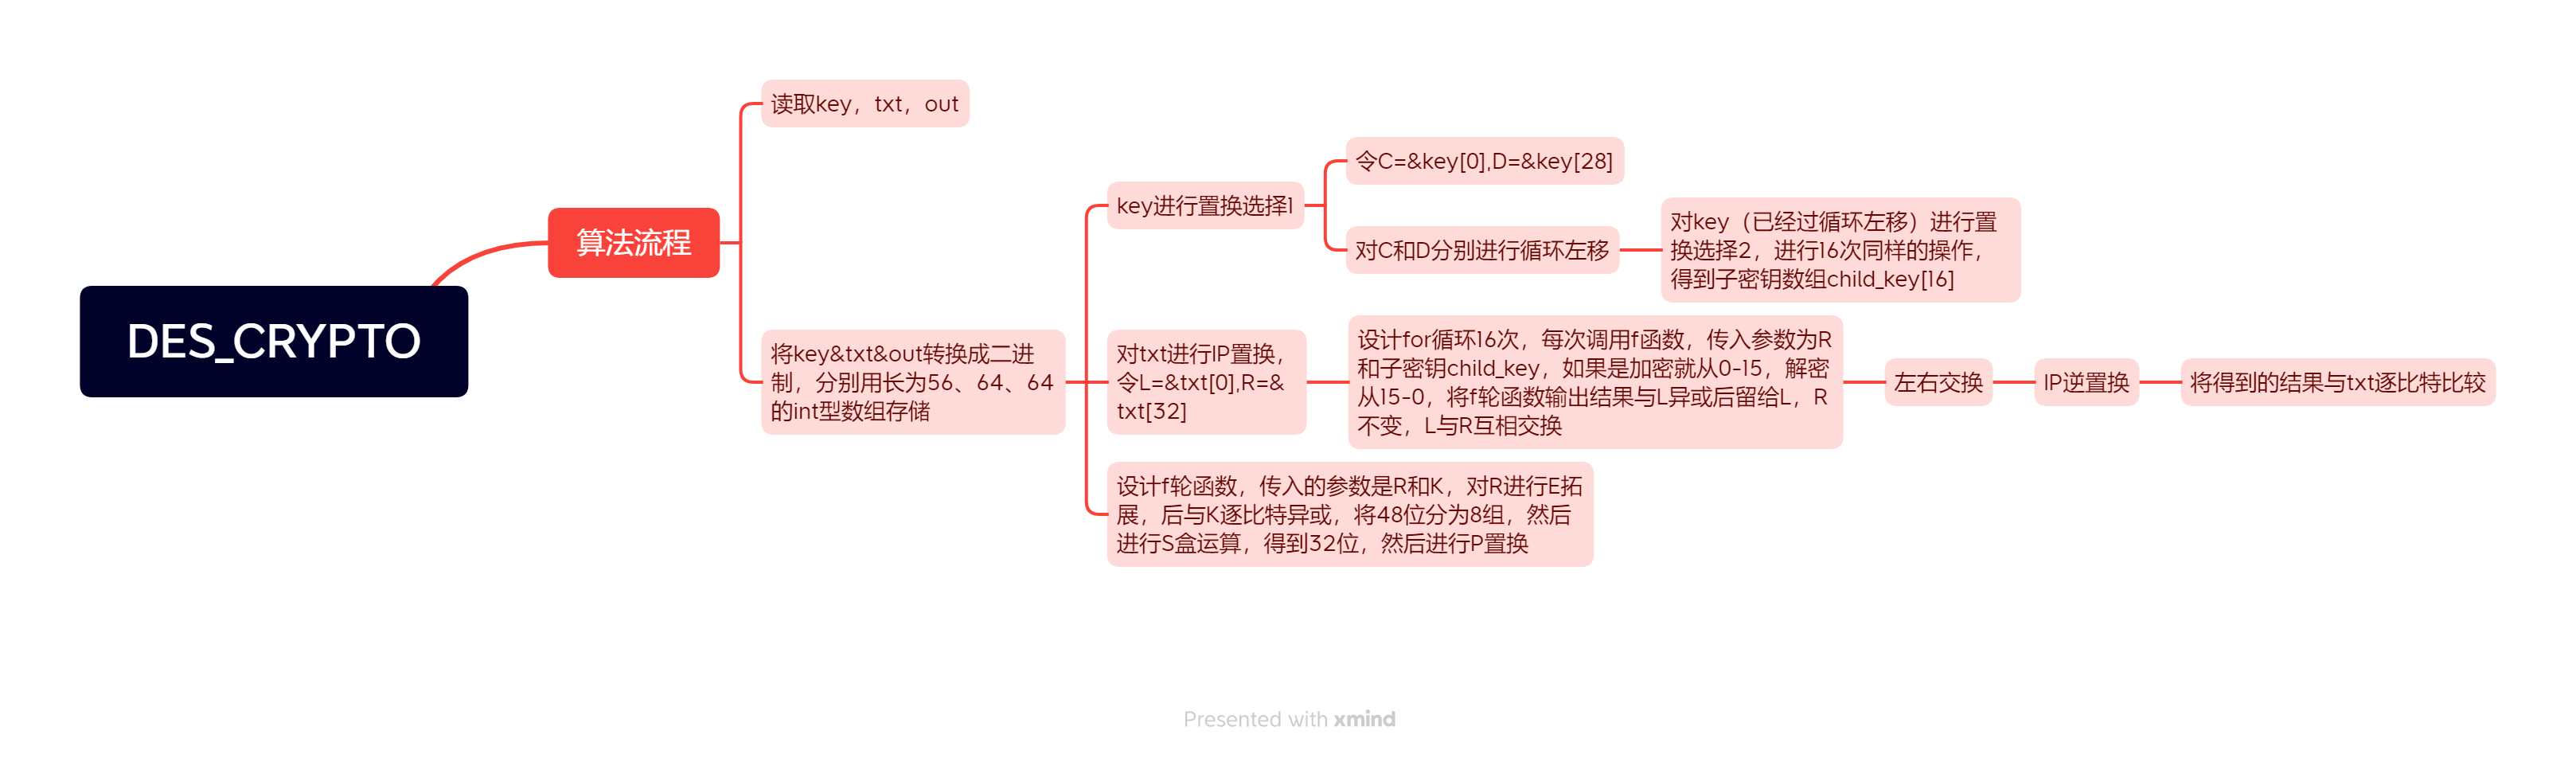
\includegraphics[height=6.8 CM]{figure/001}
%	\caption{语言处理过程图示}
%	\label{fig:语言处理过程图示}
%\end{figure}


























	\pagenumbering{arabic}
\section{字母频率统计攻击方法}

\subsection{字母频率统计攻击方法流程}
\begin{figure}[thbp!]
	\centering
	
\includegraphics[width=16cm]{figure/figure3.png}
	\caption{字母频率统计攻击方法流程}
	\label{fig:字母频率统计攻击方法流程}
\end{figure}

\subsection{字母频率统计攻击方法程序代码}
\begin{lstlisting}[language=c++]
#include <iostream>
using namespace std;
int main()
{
	char* ciphertext = new char[1024];
	cin.getline(ciphertext, 1024);
	int len = strlen(ciphertext);
	
	//统计字母频率
	int num[26], total = 0;
	for (int i = 0; i < 26; i++)
	num[i] = 0;
	for (int i = 0; i < len; i++)
	{
		if (ciphertext[i] >= 'a' && ciphertext[i] <= 'z')
		{
			int n = ciphertext[i] - 'a';
			num[n]++;
			total++;
		}
		else if (ciphertext[i] >= 'A' && ciphertext[i] <= 'Z')
		{
			int n = ciphertext[i] - 'A';
			num[n]++;
			total++;
		}
	}
	
	int n[26][2];
	for (int i = 0; i < 26; i++)
	{
		n[i][0] = i;
		cout << char('a' + i) << "的频率为:" << float(num[i]) / total << endl;
	}
	
	//将字母按频率大小排序
	for (int i = 0; i < 26; i++)
	{
		for (int j = i; j < 26; j++)
		{
			if (num[i] < num[j])
			{
				swap(num[i], num[j]);
				int temp = n[i][0];
				n[i][0] = n[j][0];
				n[j][0] = temp;
			}
		}
	}
	//for (int i = 0; i < 26; i++)
	//{
		//    //cout << num[i] << endl;
		//    cout << char(n[i][0] + 'a') << endl;
		//}
	
	//创建n[26][2]二维数组,将排好序的字母与近似字母频率一一对应起来
	//其中n[i][0]储存排好序的字母,n[i][1]储存对应的近似字母
	//然后创建temp[26]创建置换表,将字母按顺序排好
	string str = "etoiansrhlducmpyfgwbvkxjqz";
	for (int i = 0; i < 26; i++)
	{
		n[i][1] = int(str[i] - 'a');
		//cout << n[i][1] << endl;
	}
	int temp[26];
	for (int i = 0; i < 26; i++)
	{
		temp[n[i][0]] = n[i][1];
	}
	
	//校正
	swap(temp['n' - 'a'], temp['j' - 'a']);
	swap(temp['y' - 'a'], temp['f' - 'a']);
	swap(temp['d' - 'a'], temp['x' - 'a']);
	swap(temp['m' - 'a'], temp['j' - 'a']);
	swap(temp['p' - 'a'], temp['r' - 'a']);
	swap(temp['q' - 'a'], temp['h' - 'a']);
	swap(temp['z' - 'a'], temp['a' - 'a']);
	swap(temp['e' - 'a'], temp['g' - 'a']);
	swap(temp['h' - 'a'], temp['x' - 'a']);
	swap(temp['a' - 'a'], temp['e' - 'a']);
	swap(temp['o' - 'a'], temp['k' - 'a']);
	
	cout << "置换表为:" << endl;
	for (int i = 0; i < 26; i++)
	{
		cout << char(i + 'a') << " ";
	}
	cout << endl;
	for (int i = 0; i < 26; i++)
	{
		cout << char(temp[i] + 'a') << " ";
	}
	cout << endl;
	
	for (int i = 0; i < len; i++)
	{
		if (ciphertext[i] >= 'A' && ciphertext[i] <= 'Z')
		ciphertext[i] = char(temp[ciphertext[i] - 'A'] + 'a');
		else if (ciphertext[i] >= 'a' && ciphertext[i] <= 'z')
		ciphertext[i] = char(temp[ciphertext[i] - 'a'] + 'a');
	}
	cout << ciphertext << endl;
	return 0;
}
\end{lstlisting}


\subsection{程序运行结果}
\begin{figure}[H]
	\centering
	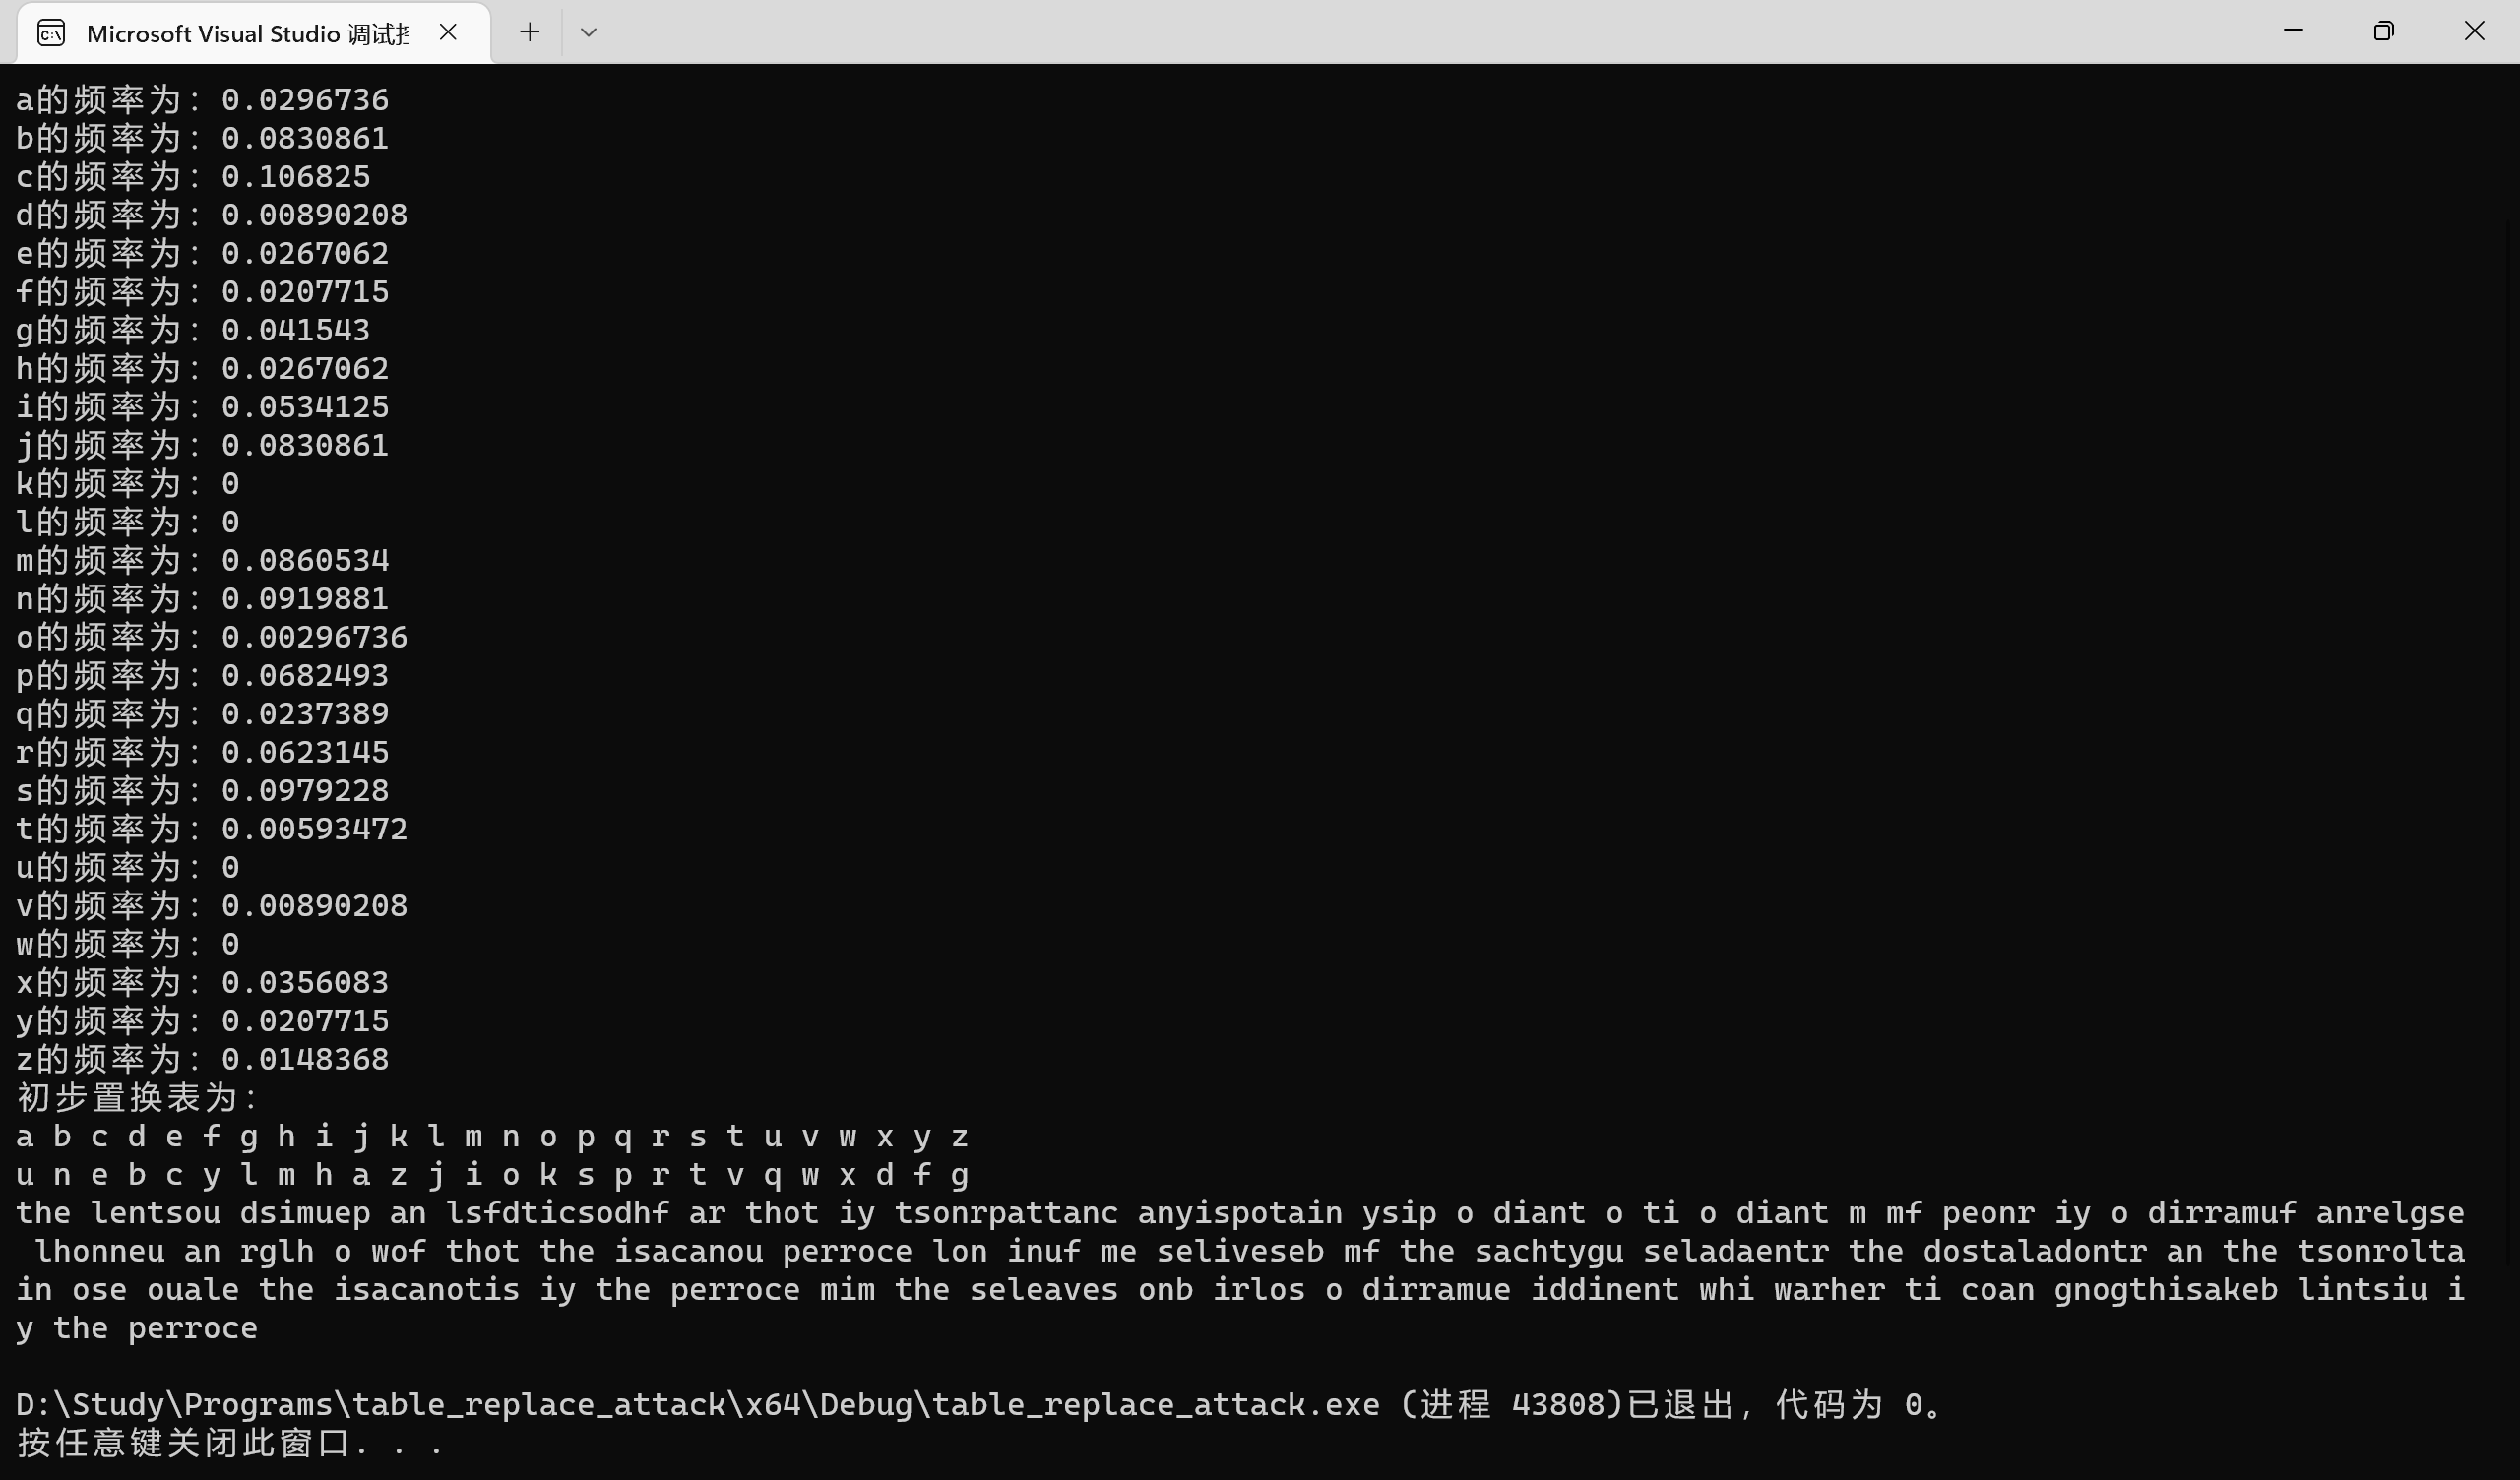
\includegraphics[width=16cm]{figure/004.png}
	\caption{字母频率统计攻击程序运行结果01}
	\label{fig:字母频率统计攻击程序运行结果01}
\end{figure}

\subsubsection{校正}
可以发现只依据单个字母的频率攻击得到的明文语义并不通顺,根据常用单词的频率

	将置换表中o、a互换\\
	置换表为:\\
	a b c d e f g h i j k l m n o p q r s t u v w x y z\\
	u n e b c y l m h o z j i a k s p r t v q w x d f g\\
	
	the lentsau dsimuep on lsfdticsadhf or that iy tsanrpottonc onyispatoin ysip a diont a ti a diont m mf peanr iy a dirromuf onrelgse lhanneu on rglh a waf that the isoconau perrace lan inuf me seliveseb mf the sochtygu selodoentr the dastolodantr on the tsanraltoin ase auole the isoconatis iy the perrace mim the seleoves anb irlas a dirromue iddinent whi worher ti caon gnagthisokeb lintsiu iy the perrace\\
	
	发现得到的明文中有"iy",应该是"if",将置换表中y、f互换\\
	
	置换表为:\\
	a b c d e f g h i j k l m n o p q r s t u v w x y z\\
	u n e b c f l m h o z j i a k s p r t v q w x d y g\\
	the lentsau dsimuep on lsydticsadhy or that if tsanrpottonc onfispatoin fsip a diont a ti a diont m my peanr if a dirromuy onrelgse lhanneu on rglh a way that the isoconau perrace lan inuy me seliveseb my the sochtfgu selodoentr the dastolodantr on the tsanraltoin ase auole the isoconatis if the perrace mim the seleoves anb irlas a dirromue iddinent whi worher ti caon gnagthisokeb lintsiu if the perrace\\
	
	发现得到的明文中有"anb",应该是"and",将置换表中b、d互换\\
	a b c d e f g h i j k l m n o p q r s t u v w x y z\\
	u n e d c f l m h o z j i a k s p r t v q w x b y g\\
	the lentsau bsimuep on lsybticsabhy or that if tsanrpottonc onfispatoin fsip a biont a ti a biont m my peanr if a birromuy onrelgse lhanneu on rglh a way that the isoconau perrace lan inuy me selivesed my the sochtfgu seloboentr the bastolobantr on the tsanraltoin ase auole the isoconatis if the perrace mim the seleoves and irlas a birromue ibbinent whi worher ti caon gnagthisoked lintsiu if the perrace\\
	
	发现得到的明文中有"ir",应该是"or",将置换表中i、o互换\\
	a b c d e f g h i j k l m n o p q r s t u v w x y z\\
	u n e d c f l m h i z j o a k s p r t v q w x b y g\\
	the lentsau bsomuep in lsybtocsabhy ir that of tsanrpittinc infospation fsop a boint a to a boint m my peanr of a borrimuy inrelgse lhanneu in rglh a way that the osicinau perrace lan onuy me selovesed my the sichtfgu selibientr the bastilibantr in the tsanraltion ase auile the osicinatos of the perrace mom the seleives and orlas a borrimue obbonent who wirher to cain gnagthosiked lontsou of the perrace\\
	
	发现得到的明文中有"frop",应该是"from",将置换表中p、m互换\\
	a b c d e f g h i j k l m n o p q r s t u v w x y z\\
	u n e d c f l p h i z j o a k r m s t v q w x b y g\\
	the lentrau bropuem in lrybtocrabhy is that of transmittinc information from a boint a to a boint p py means of a bossipuy inselgre lhanneu in sglh a way that the oricinau messace lan onuy pe relovered py the richtfgu relibients the bartilibants in the transaltion are auile the oricinator of the messace pop the releiver and oslar a bossipue obbonent who wishes to cain gnagthoriked lontrou of the messace\\
	
	
	发现得到的明文中有"py",应该是"by",将置换表中b、p互换\\
	a b c d e f g h i j k l m n o p q r s t u v w x y z\\
	g n e d l f c b h i z j o a k r m s t v q w x p y u\\
	the centrag probgem in cryptolraphy is that of transmittinl information from a point a to a point b by means of a possibgy insecure channeg in such a way that the orilinag messale can ongy be recovered by the rilhtfug recipients the participants in the transaction are agice the orilinator of the messale bob the receiver and oscar a possibge opponent who wishes to lain unauthoriked controg of the messale\\
	
	发现得到的明文中有"messale",应该是"message",将置换表中l、g互换\\
	a b c d e f g h i j k l m n o p q r s t u v w x y z\\
	l n e d g f c b h i z j o a k r m s t v q w x p y u\\
	the central problem in cryptography is that of transmitting information from a point a to a point b by means of a possibly insecure channel in such a way that the original message can only be recovered by the rightful recipients the participants in the transaction are alice the originator of the message bob the receiver and oscar a possible opponent who wishes to gain unauthoriked control of the message\\
	
	发现得到的明文中有"unauthoriked",应该是"unauthorized",将置换表中k、z互换,得到语义通顺的明文,攻击成功。\\
	置换表:\\
	a b c d e f g h i j k l m n o p q r s t u v w x y z\\
	l n e d g f c b h i k j o a z r m s t v q w x p y u\\
	the central problem in cryptography is that of transmitting information from a point a to a point b by means of a possibly insecure channel in such a way that the original message can only be recovered by the rightful recipients the participants in the transaction are alice the originator of the message bob the receiver and oscar a possible opponent who wishes to gain unauthorized control of the message\\



\begin{figure}[H]
	\centering
	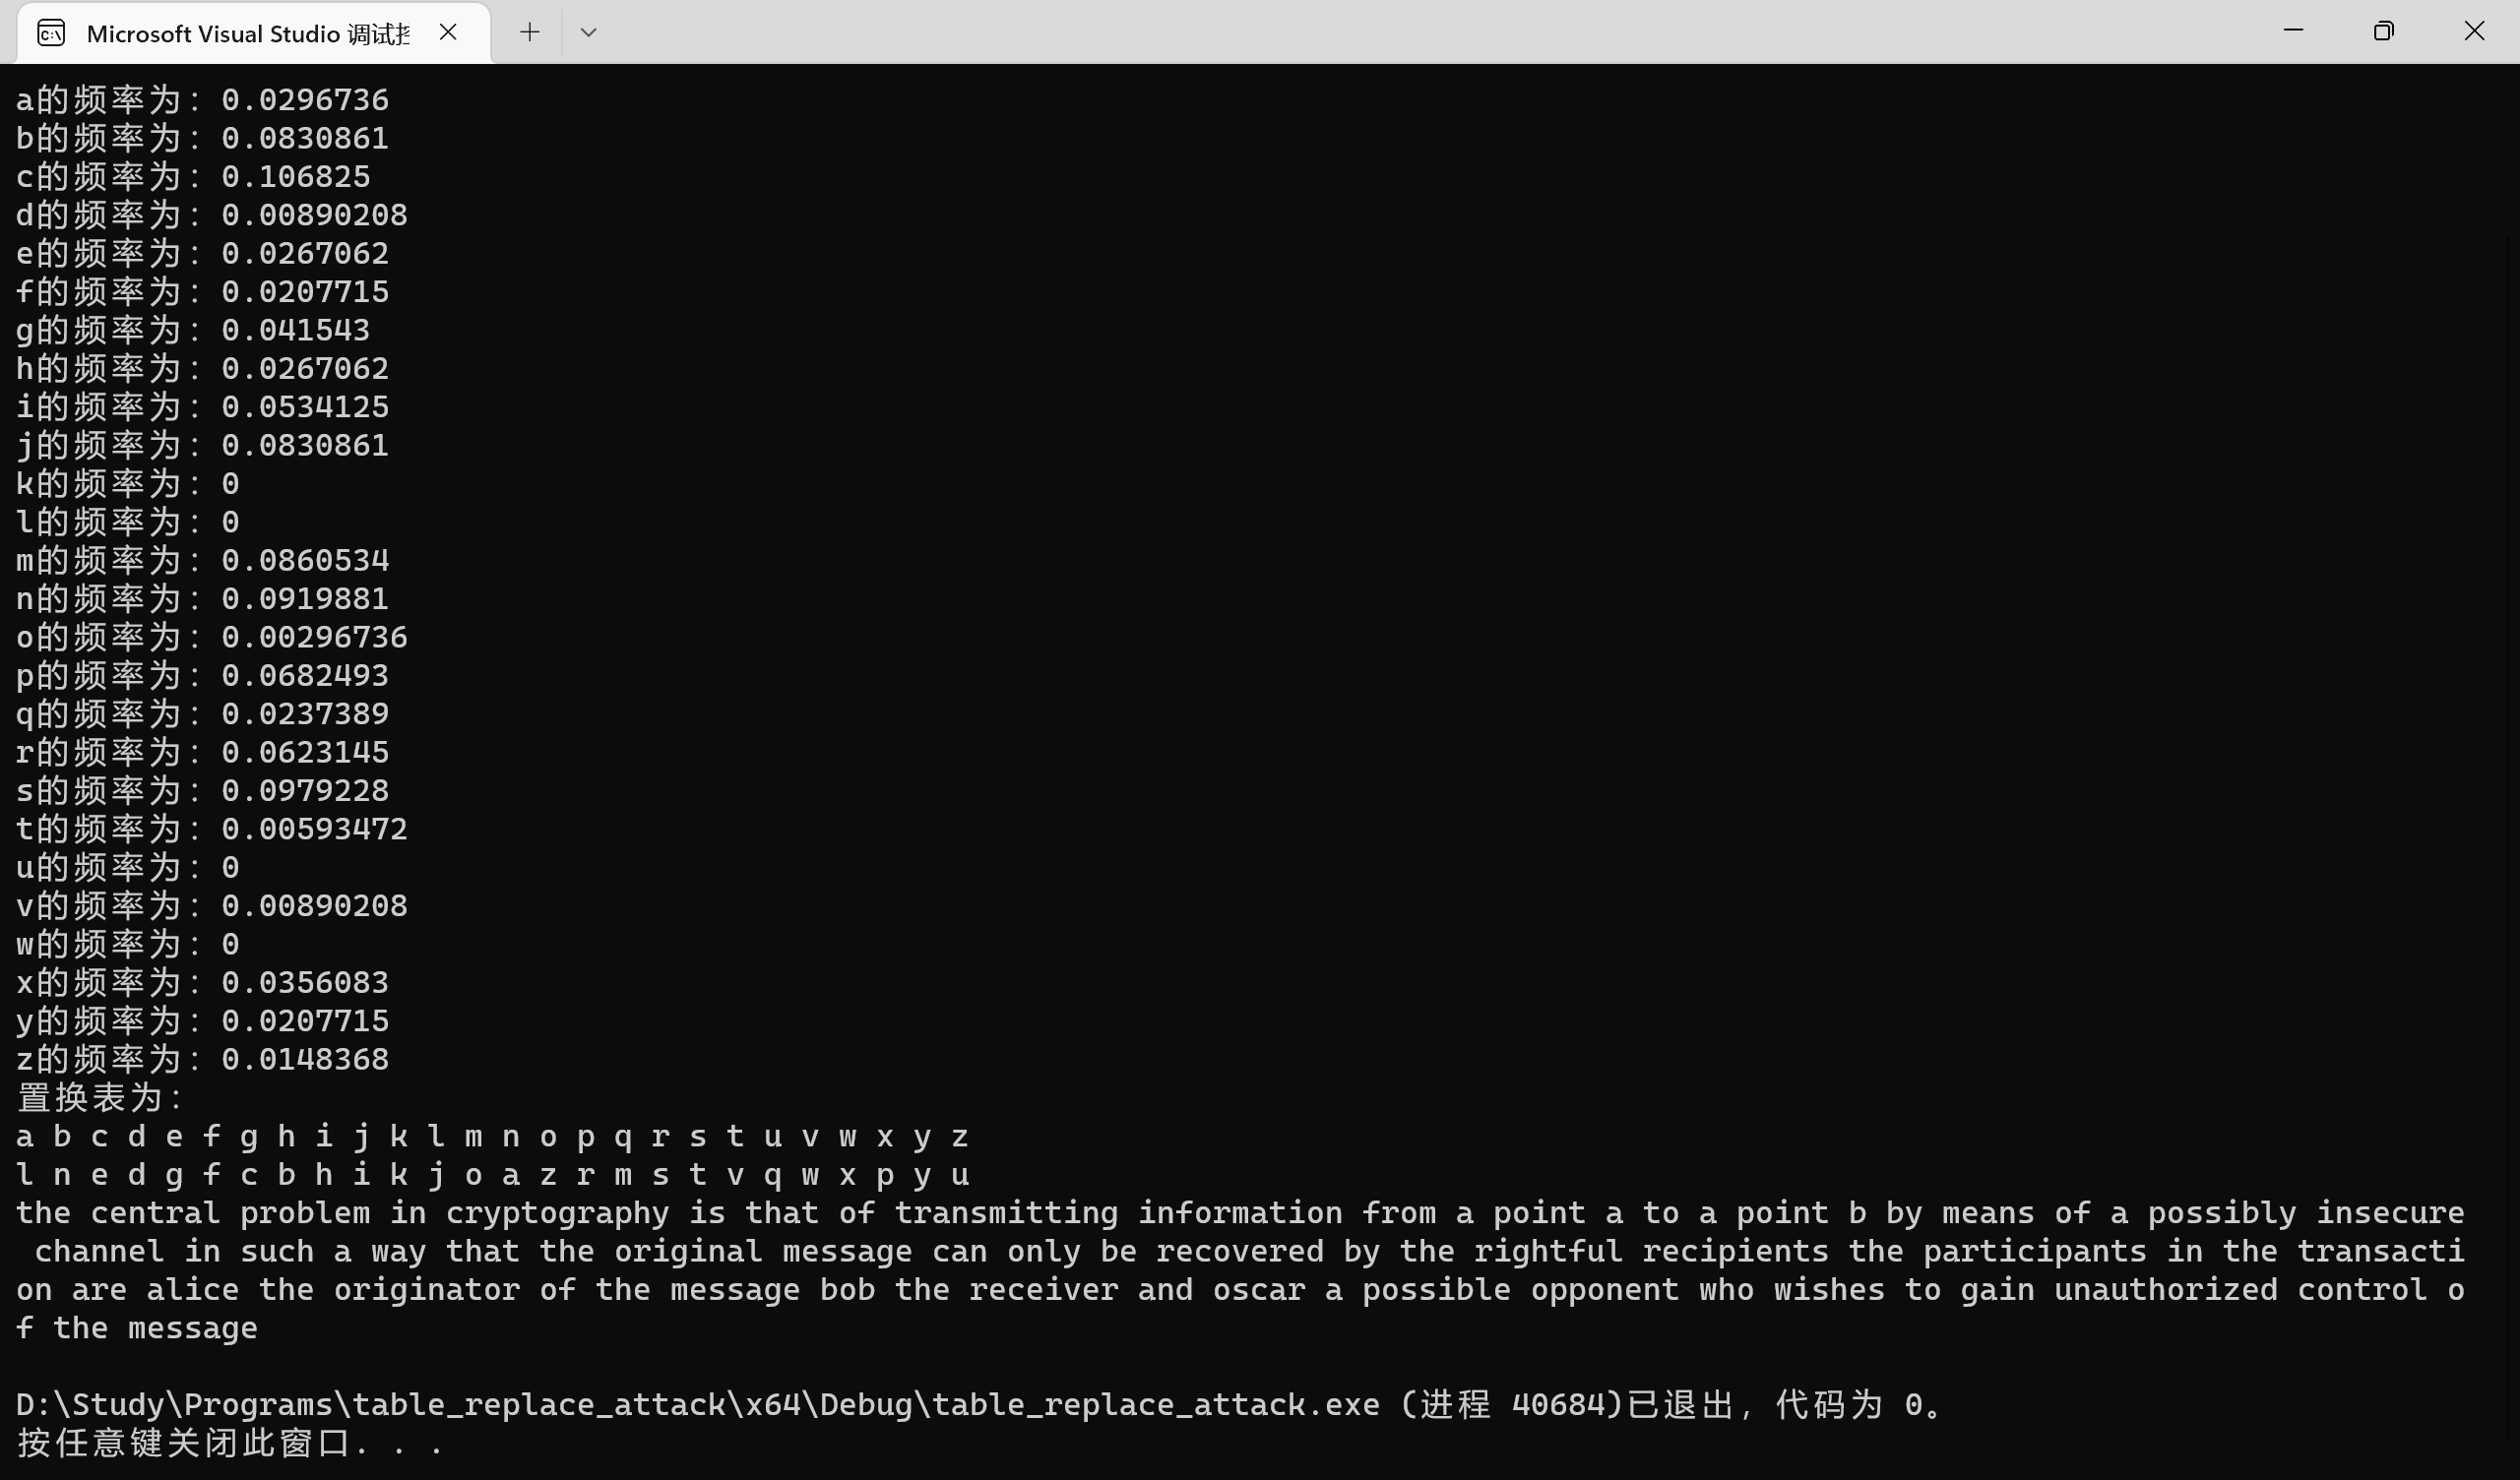
\includegraphics[width=16cm]{figure/005.png}
	\caption{字母频率统计攻击程序运行结果02}
	\label{fig:字母频率统计攻击程序运行结果02}
\end{figure}





	\section{已知问题和未来发展}
\subsection{已知问题}
本模板未采用2013版规范的页边距设置,因为实在是办不到2.5CM顶部页边距加上2.6CM的页眉设置啊。
\subsection{未来发展}
武汉理工大学本科生论文的未来发展还是需要各位用户的参与,如果每一个用户都能贡献出一点关于\LaTeX 模板的想法和意见,我相信几年之后武汉理工大学本科生论文模板会成为其他高校学习和借鉴的例子。同学当自强,让我们一起来丰富完善这个模板,如果你有很好的建议或者意见请发送到 thesis@tsaoyu.com
\subsection{官方认证}
到目前为止(\today )没有武汉理工大学任何官方组织对于本模板的格式或者内容进行认证,这代表采用本模板进行的论文写作可能不被官方的论文系统接受。如在进行原创性(防抄袭)检测的时候,可能需要提供提供doc版本的论文。希望用户了解到这个潜在的风险,做好文件转换和备份的准备。本人不对任何由于使用本模板而导致的毕业论文纠纷承担任何责任!
	%
%
%\section{汇\quad 编}
%\subsection{汇编过程概述}
%汇编(assembling)是把汇编语言代码翻译成目标机器指令的过程。\\
%
%\subsection{代码段与数据段}
%汇编阶段生成的 文件为二进制文件。目标文件由段组成,通常一个目标文件中至少有两个段:代码段和数据段。\\
%\begin{itemize}
%	\item \textbf{代码段}:代码段中包含的主要是程序的指令,代码段一般是可读可执行的,但一 般不可写。 
%	
%	\item \textbf{数据段}:数据段主要存放程序中要用到的各种全局变量或静态的数据。 数据段一般都是可读,可写,可执行的。
%\end{itemize}
%
%\subsection{例程输出分析}
%
%\subsubsection{汇编器调用命令}
%Linux中,能让GCC编译器使用编译器的输出文件test.s生成目标机器指令文件test.o的命令是:
%
%\begin{verbatim}
%      gcc test.s -c -o test.o
%\end{verbatim}
%
%其中的-c 选项表示只编译而不进行链接。
%
%\subsubsection{例程输出结果}
%
%test.s经过汇编之后得到test.o,执行过程及部分文件内容如下所示:
%
%%\begin{figure}[H]
%%	\centering
%%	\includegraphics[width=16 CM]{figure/022}
%%	\caption{汇编factorial.s生成factorial.o}
%%	\label{fig:汇编factorial.s生成factorial.o}
%%\end{figure}
%
%\begin{figure}[H]
%	\centering
%	\includegraphics[width=16 CM]{figure/0172}
%	\caption{使用UltraEdit查看test.o文件部分内容}
%	\label{fig:使用UltraEdit查看test.o文件部分内容}
%\end{figure}
%%通过 file 命令 可以查看factorial.o的文件类型:
%%\begin{verbatim}
%%      file factorial.o
%%\end{verbatim}
%%\begin{figure}[H]
%%	\centering
%%	\includegraphics[width=16 CM]{figure/024}
%%	\caption{factorial.o文件类型}
%%	\label{fig:factorial.o文件类型}
%%\end{figure}
	%\section{链\quad 接}
%\subsection{链接过程概述}
%链接(linking)是处理可重定位文件,把它们的各种符号 引用和符号定义转换为可执行文件中的合适信息的过程。而重定位是将符 号引用与符号定义进行链接的过程。\\
%
%由汇编程序生成的目标文件并不能立即就可以被执行的,其中还有许多没有 解决的问题。例如,某个源文件中的函数可能引用了另一个源文件中定义的某个变量符号,或者可能调用了某个库文件中的函数,等等。链接器的主要工作就是将有关的目标文件彼此连接,将在一个文件中引 用的符号同该符号在另外一个文件中的定义连接起来。 \\
%
%\subsection{静态链接与动态链接}
%链接处理可分为两种:静态链接和动态链接。
%\begin{itemize}
%	\item \textbf{静态链接}:静态链接过程主要是把可重定位文件依 次读入,分析各个文件的文件头,进而依次读 入各个文件的节区,并计算各个节区的虚拟内 存位置。之后,利用计算出的存储位置,对一些需要重定位的符号进行处理, 设定它们的虚拟内存地址等,最终产生一个可执行文件或者是动态链接库。 
%	
%	\item \textbf{动态链接}:动态链接所作的只是在最终的可执行程序中,记录下少量 的信息。在此可执行文件被执行时,动态链接库的全部内容将被映射虚地址空间中。动态链接程序将根据可执行程序中之前记录下来的信息找到相 应的函数指针的地址,进而能够调用这些函数,完成执行过程。 
%\end{itemize}
%
%\subsection{例程输出分析}
%
%\subsubsection{链接器调用命令}
%调用链接器生成test可执行文件的命令是:
%
%\begin{verbatim}
%      gcc test.o -o test
%\end{verbatim}
%
%\subsubsection{例程输出结果}
%
%test.o经过汇编之后得到可执行文件test,链接过程如下所示:
%
%%\begin{figure}[H]
%%	\centering
%%	\includegraphics[width=16 CM]{figure/025}
%%	\caption{链接factorial.o生成factorial}
%%	\label{链接factorial.o生成factorial}
%%\end{figure}
%
%使用如下指令可以运行test可执行文件,检验编译结果:
%\begin{verbatim}
%      ./test
%\end{verbatim}
%
%
%%\begin{figure}[H]
%%	\centering
%%	\includegraphics[width=16 CM]{figure/0252}
%%	\caption{运行test可执行文件}
%%	\label{fig:运行test可执行文件}
%%\end{figure}

	%\section{LLVM IR编程}
%\subsection{LLVM IR编程概述}
%%将源代码编译成可执行文件的过程需要四个步骤,并且还会 产生中间文件。读写文件都是 I/O 操作,而I/O将大大减慢GCC编译器完成编译的速度。\\
%%
%%pipe优化方式,会将上一步编译的结果通过管道传递给下一步。这将使得中间文件的读写全部在内存中完成,而不需要I/O操作,这将使得编译器的编译效率大幅度提升。\\
%%
%%可见,与-O优化选项不同,pipe优化选项并不是只针对编译过程中的某个阶段,而是一种整体性的编译优化。因此,在前文中没有对pipe优化进行介绍,在此用单独一节简要展示pipe优化的结果。
%LLVM IR(Intermediate Representation)是由代码生成器自顶向下遍历逐步翻译语法树形成的,
%你可以将任意语言的源代码编译成 LLVM IR,然后由 LLVM 后端对 LLVM IR 进行优化并编译为相
%应平台的二进制程序。LLVM IR 具有类型化、可扩展性和强表现力的特点。LLVM IR 是相对于 CPU指令集高级、但作为低级的代码中间表示的一种语言。从上述介绍中可以看出 LLVM 后端支持相当多
%的平台,我们无须担心操作系统等平台的问题,而且我们只需将代码编译成 LLVM IR,就可以由优化
%水平较高的 LLVM 后端来进行优化。此外,LLVM IR 本身更贴近汇编语言,指令集相对底层,能灵
%活地进行低级操作。\\
%
%%\begin{figure}[H]
%%	\centering
%%	\includegraphics[width=16 CM]{figure/0282}
%%	\caption{LLVM IR设计架构}
%%	\label{LLVM IR设计架构}
%%\end{figure}
%\subsection{例程输出分析}
%
%\subsubsection{LLVM 生成 LLVM IR命令}
%gcc命令下,生成test.ll文件的命令是:
%
%\begin{verbatim}
%     clang -S -emit-llvm test.c
%\end{verbatim}
%
%\subsubsection{例程输出结果}
%
%生成的可执行文件名为test.ll:
%
%%\begin{figure}[H]
%%	\centering
%%	\includegraphics[width=16 CM]{figure/0302}
%%	\caption{test.ll文件及注释-1}
%%	\label{test.ll文件及注释-1}
%%\end{figure}
%%\begin{figure}[H]
%%	\centering
%%	\includegraphics[width=16 CM]{figure/0312}
%%	\caption{test.ll文件及注释-2}
%%	\label{test.ll文件及注释-2}
%%\end{figure}
%%
%%检验a.out编译结果:
%%\begin{verbatim}
%%      ./a.out
%%\end{verbatim}
%%
%%
%%\begin{figure}[H]
%%	\centering
%%	\includegraphics[width=16 CM]{figure/028}
%%	\caption{运行a.out可执行文件}
%%	\label{fig:运行a.out可执行文件}
%%\end{figure}
%%
%%使用如下指令可以查看GCC编译器编译过程的耗时:
%%\begin{verbatim}
%%      g++ -ftime-report factorial.cpp (未使用pipe优化)
%%      g++ -pipe -ftime-report factorial.cpp (使用pipe优化)
%%\end{verbatim}
%%
%%\begin{figure}[H]
%%	\centering
%%	\includegraphics[width=16 CM]{figure/029}
%%	\caption{使用pipe优化与未使用pipe优化编译效率对比}
%%	\label{fig:使用pipe优化与未使用pipe优化编译效率对比}
%%\end{figure}
%%
%%同时也可以看出,是否使用pipe优化,只影响编译过程的耗时,并不会对最终的编译结果有任何影响,因为pipe优化只是改变了编译过程中中间文件的读写和存储方式,并不会给编译结果带来实质性的影响。
%%\begin{figure}[H]
%%	\centering
%%	\includegraphics[width=16 CM]{figure/030}
%%	\caption{使用pipe优化与未使用pipe优化编译结果可执行文件内容对比}
%%	\label{fig:使用pipe优化与未使用pipe优化编译结果可执行文件内容对比}
%%\end{figure}
	%============= 参考文献 =====================
	%\addcontentsline{toc}{section}{参考文献}
	%\bibliography{bibfile}
	\clearpage
	%=============  致谢  ======================
	\section*{致谢}
\addcontentsline{toc}{section}{致谢}
感谢父母为我提供的良好的衣食条件,让我有精力投入到这项没有经济回报的项目中去。
感谢徐海祥老师为我定制的论文题目,这个题目让我有兴趣制作这个模板。感谢武汉理工大学博士与硕士论文作者Hu,Weiyi,我在本模板制作的过程中参考了前辈的思路的方法。我研究过的模板还包括:上海交通大学,清华大学,哈尔滨工业大学,以及中国科技大学。其中论文引用格式GBT7714-2005-BibTeX-Style是上海财经大学的Haixing Hu作品,本模板离不开这些有益的资源的支持。同样感谢正在使用这个模板的你,相信通过你们的使用和传播,这个模板会变得越来越完善。
	%\newpage
%\appendix
%
%%%附录第一个章节
%%\section{附录1}
%
%
%%%变量列举
%
%%\begin{table}[H]
%%\caption{gcc在编译cpp文件时或g++在编译c文件和cpp文件时额外加入的宏}
%%\centering
%%\begin{tabular}{l}
%%\toprule
%%\textbf{\quad \quad \quad \quad \quad \quad 宏名称} \\
%%\midrule
%%\#define \_\_GXX\_WEAK\_\_ 1\\
%%\#define \_\_cplusplus 1\\
%%\#define \_\_DEPRECATED 1\\
%%\#define \_\_GNUG\_\_ 4\\
%%\#define \_\_EXCEPTIONS 1\\
%%\#define \_\_private\_extern\_\_ extern\\
%%\bottomrule
%%\end{tabular}
%%\end{table}
%
%
%\section{附录1}
%\textcolor[rgb]{0.98,0.00,0.00}{\quad \quad \quad \quad \quad \quad \quad \quad \quad \quad \quad \quad  \textbf{test.c源代码}}
%
%\begin{python}
%#include<stdio.h>
%int main()
%{
%	int i,n,f;
%	scanf("%d",&n);
%	i=2;
%	f=1;
%	while(i<=n)
%	{
%		f=f*i;
%		i=i+1;
%	}
%	printf("%d\n",f);
%}
%\end{python}
%
%\begin{lstlisting}[language=c++]
%#include<iostream>
%using namespace std;
%int main()
%{
%int i, n, f;
%cin >> n;
%i = 2;
%f = 1;
%while (i <= n)
%{
%%f = f * i;
%i = i + 1;
%}
%cout << f << endl;
%}
%\end{lstlisting}

	
\end{document}
%%%%%%%%%% 结束 %%%%%%%%%%